\pdfoutput=1
\pdfcompresslevel=9
\pdfinfo
{
    /Author ()
    /Title ()
    /Subject ()
    /Keywords ()
}

\batchmode
\nonstopmode

%\newcommand*{\memfontfamily}{pnc}
%\newcommand*{\memfontpack}{newcent}
\documentclass[a4paper,onecolumn,oneside,12pt]{memoir}
% Wydruk do archiwum
%\documentclass[a4paper,onecolumn,twoside,10pt]{memoir} 
%\renewcommand{\normalsize}{\fontsize{8pt}{10pt}\selectfont}
\usepackage[utf8]{inputenc}
\usepackage[T1]{fontenc}
\usepackage{setspace}
\usepackage{tabularx}
\usepackage{color,calc}
\usepackage[]{algorithm2e}
%\usepackage{soul} % pakiet z komendami do podkreślania tekstu
\usepackage{times} % pakiet zmieniający czcionki na times 

%\usepackage{longtable}
%\usepackage{ltxtable}
%\usepackage{tabulary}

\usepackage{indentfirst}
\usepackage{multicol}
\usepackage{listings}
\lstset{basicstyle=\footnotesize\ttfamily,breaklines=true}

%%%%%% Ustawienia odpowiedzialne za sposób łamania dokumentu
%\hyphenpenalty=10000		% nie dziel wyrazów zbyt często
\clubpenalty=10000      %kara za sierotki
\widowpenalty=10000  % nie pozostawiaj wdów
\brokenpenalty=10000		% nie dziel wyrazów między stronami
\exhyphenpenalty=999999		% nie dziel słów z myślnikiem
\righthyphenmin=3			% dziel minimum 3 litery

%\tolerance=4500
%\pretolerance=250
%\hfuzz=1.5pt
%\hbadness=1450

%ustawienia rozmiarów: tekstu, stopki, marginesów 
\setlength{\textwidth}{\paperwidth}
\addtolength{\textwidth}{-5cm}
\setlength{\textheight}{\paperheight}
\addtolength{\textheight}{-5cm}
\setlength{\oddsidemargin}{-0.04cm} % domyślnie jest 1 cal = 2.54 cm, stąd -0.04 da margines 2.5cm
\setlength{\evensidemargin}{-0.04cm} % domyślnie jest 1 cal = 2.54 cm, stąd -0.04 da margines 2.5cm
\topmargin -1.25cm 
\footskip 1.4cm 

\linespread{1}
%\linespread{1.3}

\usepackage{ifpdf}
%\newif\ifpdf \ifx\pdfoutput\undefined
%\pdffalse % we are not running PDFLaTeX
%\else
%\pdfoutput=1 % we are running PDFLaTeX
%\pdftrue \fi
\ifpdf
\usepackage[pdftex]{graphicx,hyperref}
\DeclareGraphicsExtensions{.pdf,.jpg,.mps,.png}
\pdfcompresslevel=9
\else
\usepackage{graphicx}
\DeclareGraphicsExtensions{.eps,.ps,.jpg,.mps,.png}
\fi
\sloppy

%\graphicspath{{rys01/}{rys02/}}
%\usepackage{rotating}

\renewcommand{\topfraction}{1.0}
\renewcommand{\bottomfraction}{1.0}
\renewcommand{\textfraction}{0.0}
\renewcommand{\floatpagefraction}{0.35}

%%%%%%%%%%%%%%%%%%%%%%%%%%%%%%%%%%%%%%%
%                  Definicja strony tytułowej 
%%%%%%%%%%%%%%%%%%%%%%%%%%%%%%%%%%%%%%%
\makeatletter
%Uczelnia
\newcommand\uczelnia[1]{\renewcommand\@uczelnia{#1}}
\newcommand\@uczelnia{}
%Wydział
\newcommand\wydzial[1]{\renewcommand\@wydzial{#1}}
\newcommand\@wydzial{}
%Kierunek
\newcommand\kierunek[1]{\renewcommand\@kierunek{#1}}
\newcommand\@kierunek{}
%Specjalność
\newcommand\specjalnosc[1]{\renewcommand\@specjalnosc{#1}}
\newcommand\@specjalnosc{}
%Tytuł po angielsku
\newcommand\titleEN[1]{\renewcommand\@titleEN{#1}}
\newcommand\@titleEN{}
%Tytuł krótki
\newcommand\titleShort[1]{\renewcommand\@titleShort{#1}}
\newcommand\@titleShort{}
%Promotor
\newcommand\promotor[1]{\renewcommand\@promotor{#1}}
\newcommand\@promotor{}

\def\maketitle{%
  \null
  \pagestyle{empty}%i
	{\centering\vspace{-1cm}
		{\fontsize{22pt}{24pt}\selectfont \@uczelnia}\\[0.4cm]
		{\fontsize{22pt}{24pt}\selectfont \@wydzial }\\[0.5cm]
		\hrule \vspace*{0.7cm}
	}
{\flushleft\fontsize{14pt}{16pt}\selectfont%
\begin{tabular}{ll}
KIERUNEK: & \@kierunek\\
SPECJALNOŚĆ: & \@specjalnosc\\
\end{tabular}\\[1.3cm]
}
{\centering
\vskip 1cm
{\fontsize{24pt}{26pt}\selectfont PRACA DYPLOMOWA}\\[0.5cm]
{\fontsize{24pt}{26pt}\selectfont MAGISTERSKA}\\[2cm]
%{\fontsize{24pt}{26pt}\selectfont PROJEKT INżYNIERSKI}\\[1.5cm]
\vskip 0.8cm
}
%
\begin{tabularx}{\linewidth}{p{6cm}>{\centering\arraybackslash}X}
		&{\fontsize{16pt}{18pt}\selectfont \@titleEN}\\[5mm] 	%UWAGA: tutaj jest miejsce na tytył w języku polskim
		&{\fontsize{16pt}{18pt}\selectfont \@title}\\[10mm] %UWAGA: tutaj jest miejsce na tytył w języku angielskim
\end{tabularx}
\vfill
\begin{tabularx}{\linewidth}{p{6cm}l}
		%UWAGA: tutaj jest miejsce na autora pracy
		&{\fontsize{16pt}{18pt}\selectfont AUTOR:}\\[5mm]
		&{\fontsize{14pt}{16pt}\selectfont \@author}\\[10mm]
		%UWAGA: tutaj jest miejsce na promotora pracy 
		&{\fontsize{16pt}{18pt}\selectfont PROWADZĄCY PRACĘ:}\\[5mm]
		&{\fontsize{14pt}{16pt}\selectfont \@promotor}\\[10mm]
		&{\fontsize{16pt}{18pt}\selectfont OCENA PRACY:}\\[20mm]
	\end{tabularx}
\hrule\vspace*{0.3cm}
{\centering
%{\fontsize{24pt}{26pt}\selectfont PRACA DYPLOMOWA}\\[0.5cm]
%{\fontsize{24pt}{26pt}\selectfont MAGISTERSKA}\\[2cm]
{\fontsize{16pt}{18pt}\selectfont \@date}\\[0cm]
}
\normalfont
 \cleardoublepage
}
\makeatother
%%%%%%%%%%%%%%%%%%%%%%%%%%%%%%%%%%%%%%%
%                  Styl rozdziałów 
%%%%%%%%%%%%%%%%%%%%%%%%%%%%%%%%%%%%%%%
\setcounter{secnumdepth}{3}
\setcounter{tocdepth}{3}
%\definecolor{niceblue}{rgb}{.168,.234,.671}

%\AtBeginDocument{% 
%        \addto\captionspolish{% 
%        \renewcommand{\tablename}{Table}% 
%}%} 

%\AtBeginDocument{% 
%        \addto\captionspolish{% 
%        \renewcommand{\chaptername}{Rozdział}% 
%}} 

%\AtBeginDocument{% 
%        \addto\captionspolish{% 
%        \renewcommand{\figurename}{Image}% 
%}%}
%        \addto\captionspolish{% 
%        \renewcommand{\bibname}{Literature}% 
%}


%%%%%%%%%%%%%%%%%%%%%%%%%%%%%%%%%%%%% nowe itemize
\makeatletter
\renewenvironment{itemize}{
  \begin{list}{  
  \csname labelitem\romannumeral\the\@listdepth\endcsname}{
  \setlength{\leftmargin}{1em}
	\setlength{\topsep}{6pt}%
	\setlength{\partopsep}{0pt}%
	\setlength{\parskip}{0pt}%
	\setlength{\parsep}{0pt}%
	\setlength{\itemsep}{0pt}}
}{
  \end{list}
}

%%%%%%%%%%%%%%%%%%%%%%%%%%%%%%%%%%%%%%%%%%%%%%%%%%%%%%%%%%%%%%%%%% Styl wyliczenia (opis skrótów) 
%%%%%%%%%%%%%%%%%%%%%%%%%%%%%%%%%%%%%%%%%%%%%%%%%%%%%%%%%%%%%%%%%
\newenvironment{Ventry}[1]%
 {\begin{list}{}{\renewcommand{\makelabel}[1]{\textbf{##1}\hfill}%
   \settowidth{\labelwidth}{\textbf{#1}}%
   \setlength{\leftmargin}{3cm}}}%
 {\end{list}}

\addtopsmarks{headings}{%
\nouppercaseheads % added at the beginning
}{%
\createmark{chapter}{both}{shownumber}{}{. \space}
%\createmark{chapter}{left}{shownumber}{}{. \space}
\createmark{section}{right}{shownumber}{}{. \space}
}%use the new settings
\pagestyle{headings}

\newlength\mytemplengtha

\setcounter{secnumdepth}{2}
\setcounter{tocdepth}{2}
\setsecnumdepth{subsection} % activating subsubsec numbering in doc

\makeatletter
\copypagestyle{outer}{headings}
\makeoddhead{outer}{}{}{\slshape\rightmark}
\makeevenhead{outer}{\slshape\leftmark}{}{}
\makeoddfoot{outer}{\@author:~\@titleEN}{}{\thepage}
\makeevenfoot{outer}{\thepage}{}{\@author:~\@titleEN}
\makeheadrule{outer}{\linewidth}{\normalrulethickness}
\makefootrule{outer}{\linewidth}{\normalrulethickness}{6pt}
\makeatother

% fix plain
%\copypagestyle{plain}{outer} % overwrite plain with outer
\makeoddhead{plain}{}{}{} % remove right header
\makeevenhead{plain}{}{}{} % remove left header
\makeevenfoot{plain}{}{}{}
\makeoddfoot{plain}{}{}{}

%\copypagestyle{plain}{outer} % overwrite plain with outer
\makeoddhead{empty}{}{}{} % remove right header
\makeevenhead{empty}{}{}{} % remove left header
\makeevenfoot{empty}{}{}{}
\makeoddfoot{empty}{}{}{}

\pagestyle{outer}

%definicja nagłówków
%\renewcommand{\chaptermark}[1]{\markboth{\ifnum \c@secnumdepth >\z@ \thechapter \ \fi #1}{}} 
%\renewcommand{\chaptermark}[1]{\markboth{\thechapter \ #1}{\thesection \ #1}} 
%\renewcommand{\sectionmark}[1]{\markright{\thesection \ #1}{}} 
%\renewcommand{\chaptermark}[1]{\markboth{\thechapter \MakeUppercase{#1}}{}}

%kropki po numerach sekcji
\makeatletter
\def\@seccntformat#1{\csname the#1\endcsname.\quad}
\def\numberline#1{\hb@xt@\@tempdima{#1\if&#1&\else.\fi\hfil}}
\makeatother

\renewcommand{\chapternumberline}[1]{#1.\quad}
\renewcommand{\cftchapterdotsep}{\cftdotsep}

%\AtBeginDocument{\addtocontents{toc}{\protect\thispagestyle{empty}}}

%\includeonly{wstep,rozdzial01} % jeśli chcemy kompilować tylko fragmenty, to można tu je wpisać
%%%%%%%%%%%%%%%%%%%%%%%%%%%%%%%%%%%%%%%%%
%                  Początek dokumentu 
%%%%%%%%%%%%%%%%%%%%%%%%%%%%%%%%%%%%%%%%%
\begin{document}
\title{Filtracja i segmentacja drukowanych w kolorze obrazów}
\titleShort{Filtracja i segmentacja drukowanych w kolorze obrazów}
\titleEN{Preprocessing and segmentation of color-printed images}
\author{Marcin Wojciechowski}
\uczelnia{POLITECHNIKA WROCŁAWSKA}
\wydzial{WYDZIAŁ ELEKTRONIKI}
\kierunek{INFORMATYKA}
\specjalnosc{Internet Engineering}
\promotor{dr inż. Tomasz Babczyński}
\date{WROCŁAW, 2014}
\maketitle

\pagestyle{outer}
\mbox{}\pdfbookmark[0]{Table of Contents}{spisTresci.1}
\tableofcontents* 
\newpage

\chapter{Introduction}

Beginning of this chapter is focused on the problem background. Next part is focused on a 
full description of the topic and definition of main objectives of this thesis.
In the last part of this chapter there is a full structure of this document given.

\section{Background}

Nowadays image digitization is a very important topic. It has a lot of practical applications.
For example, it is a very good way to prevent destruction of old photos,
to archive them (to keep them in one place in a digital version) and make it easier to 
send a picture from one place to another. Unfortunately, basic method of image digitization - 
scanning - has some disadvantages. Due to errors made during a scanning procedure,
input image distortions or quality of a scanning device, resulting digitized images 
have a poor quality. This issue is a great motivation to research in a field of digital image
processing. To improve digitization process there are many filtration algorithms,
which task is to solve this problem and to produce an image with better quality.

Image digitization has another big advantage - there is a possibility to retrieve information from
the picture (for example: pattern recognition, feature extraction). This feature is handled by
segmentation algorithms. Although this group is one of the most difficult in image processing, there
is a big emphasis on a research, due to many advantages of this type of algorithms in practical
use. \\

Digital image processing can be optimized to work with special types of the images. This work 
focuses on improval of color-scanned maps quality. It is a very interesting topic, because maps
processed with this kind of the algorithm can be used as an input for further map analysis by other 
applications, to improve their readability or to allow them to edit.

\section{Problem statement and main objectives}

The main aim of this thesis is to create a filtration and segmentation algorithm, which should apply
to scanned color-printed images. This work is focused on scanned maps. Resulting algorithm should be
optimized to use it with this type of scanned images. Output image should have following properties:

\begin{itemize}
  \item most of distortions should be eliminated;
  \item image should be divided into consistent areas, like forests, lakes, rivers, etc. These areas
        should be marked on the map in a consistent way (it should have the same color);
  \item detected areas should have the same size like in an input image;
  \item small details, like text should be kept and marked in a resulting image.
\end{itemize}

Used fltering algorithms should remove main distortions and all disadvantages of image scanning (like
for example rasters, moro effect). Next, proper segmentation algorithm should be used to detect all
areas in an input map and to divide the map into different, homogenous regions. \\

The final solution - set of algorithms - should be impemented in a chosen programming language.
Created application should be tested on many different scanned maps. Finally, test results should be
analysed.

\section{Document structure}

This document has been divided into six chapters and the bibliography at the end.
Below there is a short description of a content of each chapter:

\begin{itemize}
  \item In the first chapter there is a description and the background of the topic.
        Next there are listed main objectives of the work and a problem statement;
  \item In the second chapter there is a theoretical introduction of the problem. There are
        explained all already known filtration and segmentation algorithms used in this work.
        The description consists of the definition, properties and parameters of each method. In the
        second part, there is an analysis of existing research work and solutions of the color
        scanned maps preprocessing problem;
  \item Third chapter focuses on the research part of this thesis. There are listed all found problems,
        which should be taken into consideration in the analysis of color scanned maps.
  \item In the fourth chapter there is a full description of filtration and segmentation algorithms
        designed in this work;
  \item Fifth chapter focuses on the engineering part of the thesis. There is a description of all
        implementation details of the algorithm;
  \item In the sixth chapter there are described all tests of developed algorithm. In the second part
        there are test results with proper analysis given;
  \item In the last chapter there are conclusions of the thesis.
\end{itemize}

\chapter{Theoretical introduction}

This section contains all definitions and concepts needed for a good understanding of the work. It
also covers history and basic usage of digital image processing. The last section is focused on
actual state of art in the topic of filtration and segmentation of color printed digital images.

\section{Digital image processing}

\subsection{History and usage}

According to \cite{digitalImageProcessing},
digital image processing has a lot of practical applications. It was used first at the beginning of
the XX century to send pictures over long distances. Research and development of digital image
processing algorithms  was strongly associated with growth of the computer industry. It was caused
by high computational complexity of this type of algorithms. Further growth began in 1960s. Many 
techniques were developed in organisations like Jet Propulsion Laboratory, Massachusetts Institute
of Technology or Bell Laboratories. It was used in satellite imagery, medical imaging (in 1970s 
computerized tomography was developed), image enhancement, science (for example in geography - 
in research about pollution, archeology - in restoring blured pictures), defence or industry.
Another area of digital image processing focuses on extracting of an information from the picture in
a form suitable for the computer processing. It is used in a character recognition (OCR), industry (
automatic inspection of production process), military, forensics (recognition of fingerprints) and
weather prediction. \\

Nowadays, with fast computers and signal processors, digital image processing is used widely.
It is mainly caused by its low price and versatility.

\subsection{Basic definitions}

A digital image can be defined as a two dimentional function f(x, y), where x and y denote spatial 
coordinates and f(x, y) is the intensity or gray level of the image at this point. Values of x, y
and f(x, y) should be finite and descrete quantities. Digital image processing refers to processing 
digital images by means of a digital computer. It includes many primitive operations like noise
reduction, contrast enhancement or image sharpening. It also involves more advanced algorithms like
image segmentation (partitioning an image into regions or objects), description of objects,
classification (recognition) of objects and even advanced analysis of an image. Digital image 
processing algorithms take an image as an input. Output depends on a type of the algorithm.
It can be new, processed image or a group of attributes taken from an image. Main tasks of digital
image processing are:

\begin{itemize}
  \item Image aquisition;
  \item Image enhancement;
  \item Image restoration;
  \item Wavelets;
  \item Compression;
  \item Feature extraction;
  \item Segmentation;
  \item Recognition.
\end{itemize}

This work focuses mainly on image enhancement and image segmentation. All algorithms used in this 
work are described in next sections.

\section{Image enhancement}

Image enhancement algorithms are one of the simplest and most commonly used group of digital image
processing. Main idea of those algorithms is to improve image quality, bring out obscured details 
or highlight certain features of an image. The main aim of image enhancement is to process image 
and return it in a more suitable form, than input for a specific application. Proper image enhancement
algorithms should be chosen for different cases (algorithm solving one problem may be inadequate for
other problems). Image enhancement algorithms can be divided into two groups:

\begin{itemize}
  \item Spatial domain - manipulation of pixels of an image directly;
  \item Frequency domain - modification of Fourier transform of an image.
\end{itemize}

\subsection{Smoothing algorithms}

According to \cite{learningOpenCv}, smoothing is a very simple and frequently applied operation. It
is used to reduce noise or camera artifacts and also in the image resolution reduction. In this work
there are two smoothing algorithms applied.

\subsubsection{Gaussian blur}

Gaussian filter is one of the most frequently used filters. According to \cite{learningOpenCv}, 
gaussian blur is done by convolving each point in the input array with a Gaussian kernel and then
summing to produce the output array. Resulting image is a smooth blur. It is used to reduce noise
or image details and as a part of edge detection algorithms. Algorithm has two parameters:

\begin{itemize}
  \item \textit{Radius} - it is a kernel size. The bigger value set, the smoother is image;
  \item \textit{Standard Deviation} in X and Y direction.
\end{itemize}

Example result of a Gaussian Blur filter application is shown in a Fig.~\ref{gaussianBlurExample}.

\begin{figure}[!ht]
\begin{center}
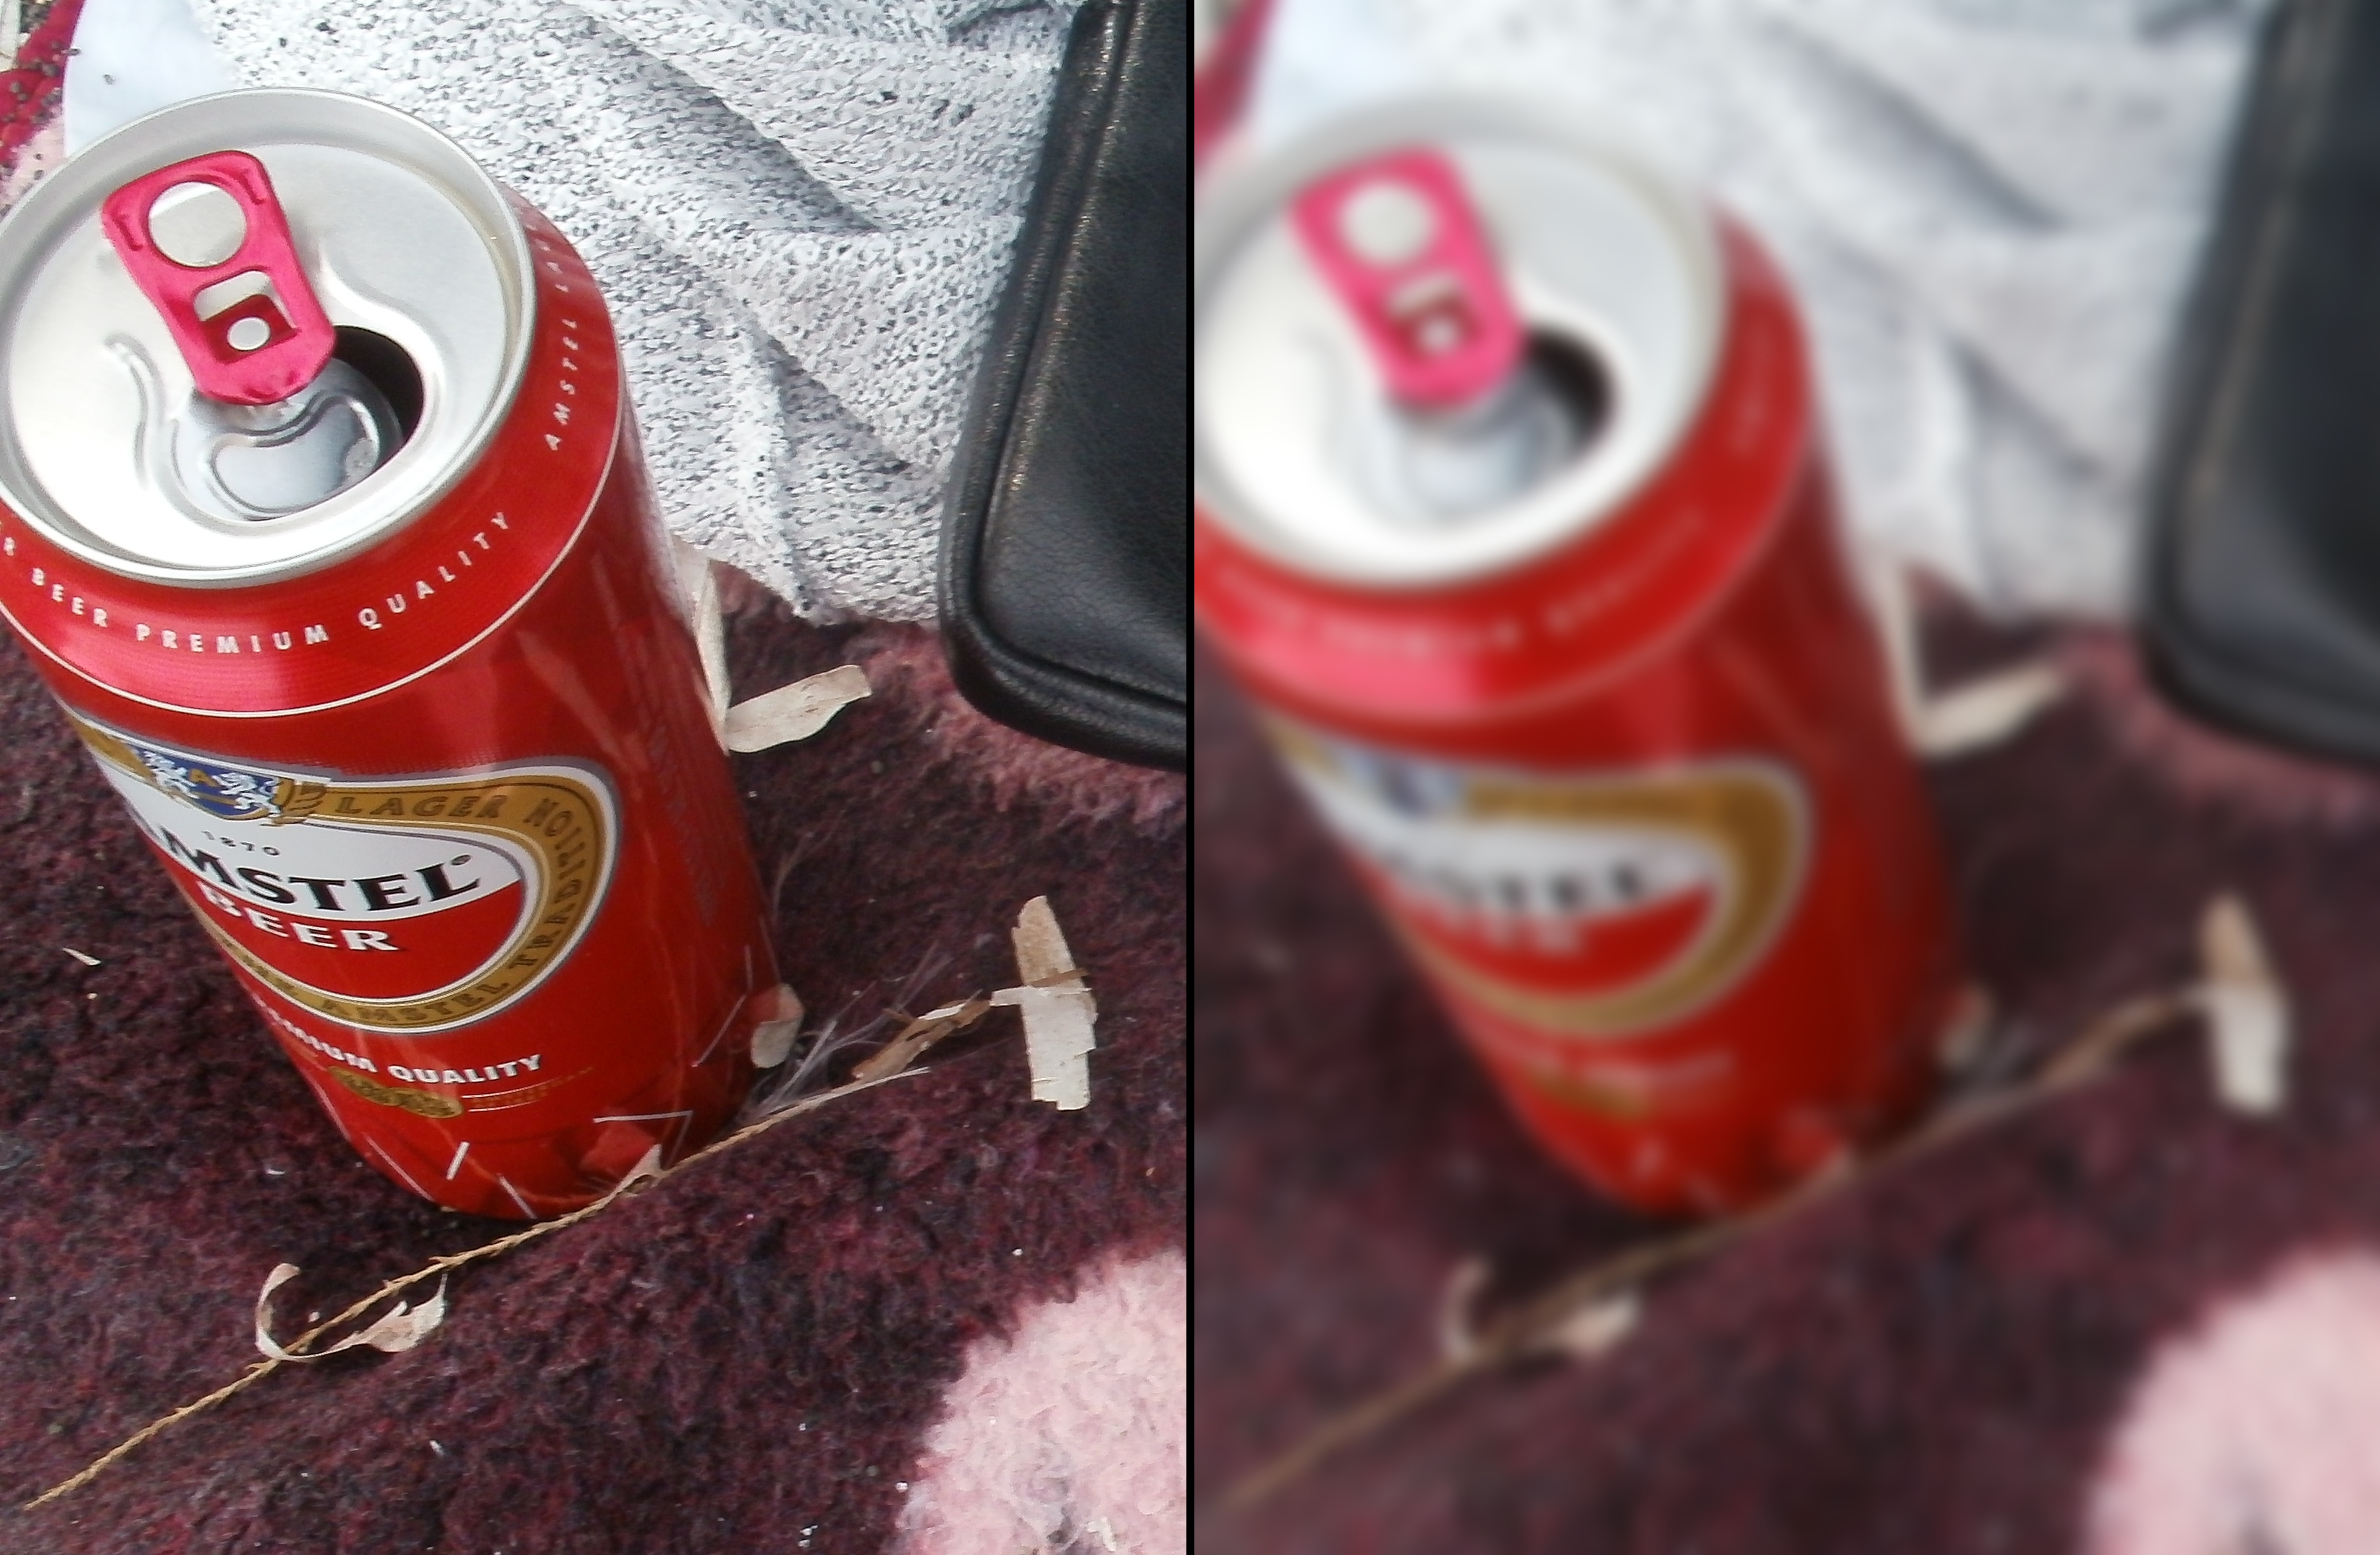
\includegraphics[scale=0.1]{images/GaussianBlurExample.jpg}
\caption{Gaussian Blur example. \\
Source: own}
\label{gaussianBlurExample}
\end{center}
\end{figure}

\subsubsection{Bilateral filter}

According to \cite{bilateralFilterWiki}, bilateral filter is a non-linear, edge-preserving and
noise reducing filter for images. The intensity value at each pixel in an image is replaced by a
weighted average of an intensity values from nearby pixels. In contrast to the Gaussian Blur, 
weights are based on the difference of intensity from the center pixel. This algorithm is commonly
used to prepare an input for segmenting algorithms. Algorithm takes three parameters:

\begin{itemize}
  \item \textit{Diameter} of each pixel that is used during filtering. For larger values of 
        parameters, the algorithm is slower and takes into consideration larger pixel surrounding;
  \item \textit{Filter Sigma in a color space}. A larger value of this parameter means, that farther
        colors within the pixel neighborhood will be mixed together. Resulting image will have
        larger areas with semi-equal color;
  \item \textit{Filter Sigma in the coordinate space}. A larger value of the parameter means that
        farther pixels will influence each other as long as their colors are close enough.
\end{itemize}

Example of a bilateral filter usage is presented in a fig.~\ref{bilateralFilterExample}.

\begin{figure}[!ht]
\begin{center}
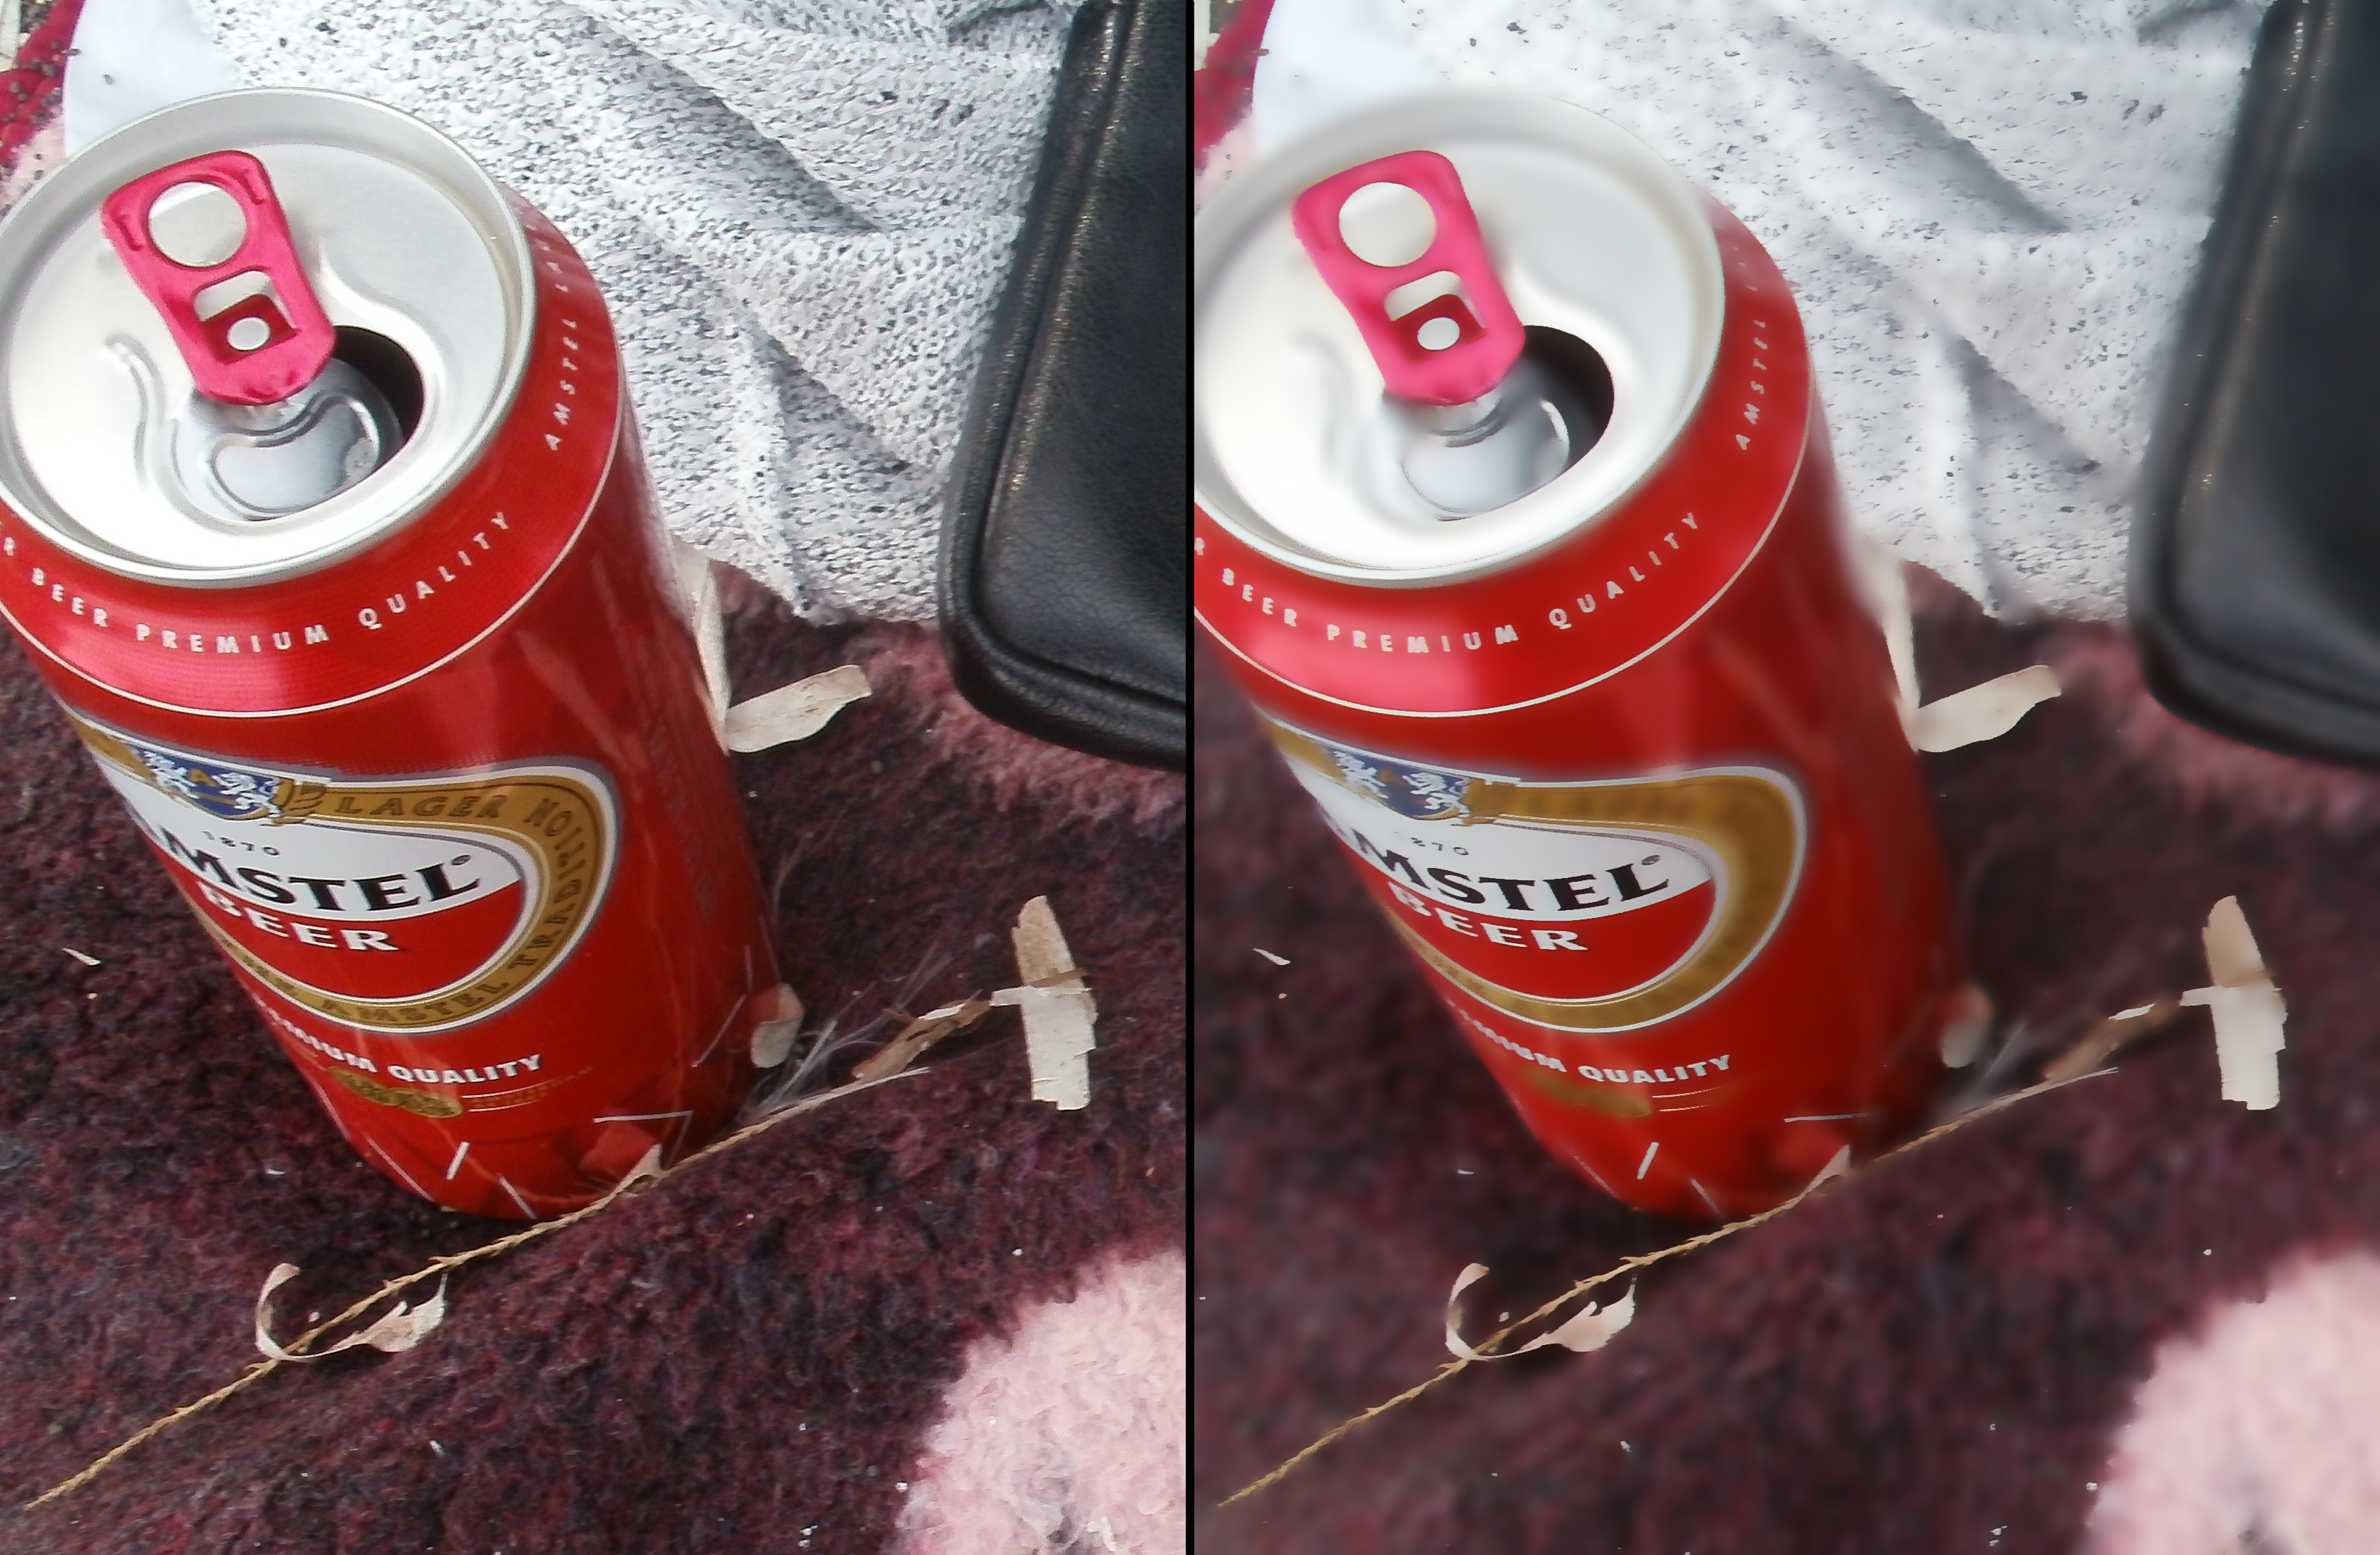
\includegraphics[scale=0.1]{images/BilateralFilterExample.jpg}
\caption{Bilateral Filter example. \\
Source: own}
\label{bilateralFilterExample}
\end{center}
\end{figure}

\subsection{Morphological transformations}

Morphological operations are used to remove noise, isolate or join disparate elements in an image 
and to find intensity bumps or holes in an image to aquire image gradients. Basic  morphological
operations are called Dilation and Erosion.

\subsubsection{Dilation}

Dilation is a convolution of an image with a kernel. The kernel can have any shape or size and has
to have defined an anchor point. When kernel is scanned over the image, there is computed maximum
pixel value covered by the kernel. Then, the anchor point value is set to maximum value. Dilation
causes growth of all bright elements in an image. Example of dilation is presented in a
Fig.~\ref{dilationExample}

\begin{figure}[ht]
\begin{center}
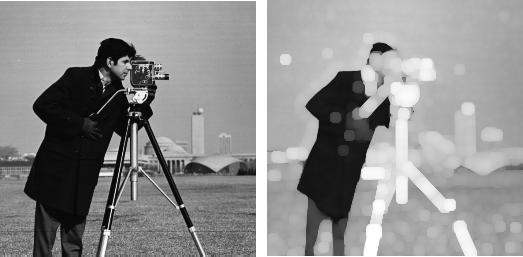
\includegraphics[scale=0.6]{images/dilationExample.jpg}
\caption{Dilation example. \\
Source: http://www.mathworks.com/help/images/ref/referenceipart130.gif}
\label{dilationExample}
\end{center}
\end{figure}

\subsubsection{Erosion}

Erosion is a converse operation to dilation. Main difference is that it computes local minimum over
the area of the kernel. Erosion causes growth of all dark elements in an image. Example of erosion
is presented in Fig.~\ref{erosionExample}

\begin{figure}[ht]
\begin{center}
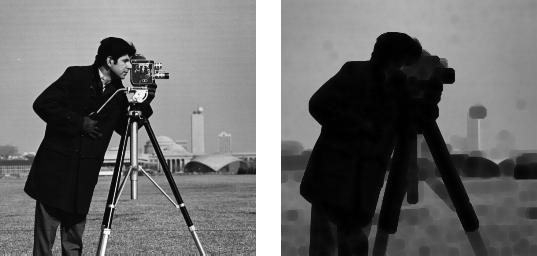
\includegraphics[scale=0.6]{images/erosionExample.jpg}
\caption{Erosion example. \\
Source: http://www.mathworks.com/help/images/ref/referenceipart128.gif}
\label{erosionExample}
\end{center}
\end{figure}

Dilation and erosion take two parameters:

\begin{itemize}
  \item \textit{Size of rectangular structuring element used for erosion/dilation}. If it is set to
        3, the structuring element is a matrix with size 3x3. The bigger value is set, the stronger
        impact has the algorithm on the image;
  \item \textit{Number of iterations} of the algorithm.
\end{itemize}

\subsection{Denoising}

Main goal of this type of algorithms is to eliminate noise from the image. In this work it is used 
Non-local Means Denoising algorithm \cite{nonLocalMeansDenoising}. This filter takes one argument.
It regulates the strength of a filter. Big value of the parameter perfectly removes noise but also
removes image details. Smaller parameter values preserve details but also preserve some noise.
Example of its usage is presented in a Fig.~\ref{denoisingExample}.

\begin{figure}[ht]
\begin{center}
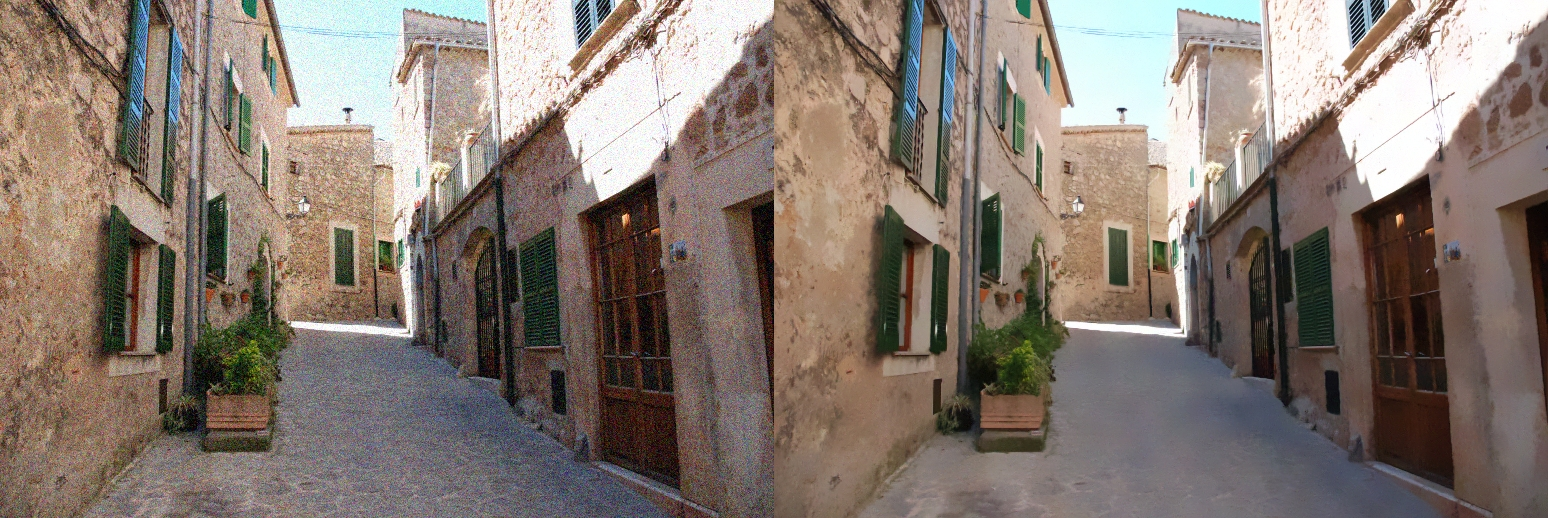
\includegraphics[scale=0.3]{images/denoisingExample.jpg}
\caption{Denoising example. \\
Source: Image generator in \cite{nonLocalMeansDenoising}}
\label{denoisingExample}
\end{center}
\end{figure}

\subsection{Unsharp mask}

Unsharp mask is applied to highlight or enhance some details of the image. According to 
\cite{unsharpMaskWiki}, this technique uses a blured or unsharped image to create mask of the
original image. The unsharped mask is then combined with the negative image. As a result there is an
image less blurry than the original. In the algorithm used in this work, Gaussian blur is used and
then its result is compared to the original image. If the difference is greater than specified
threshold value, images are subtracted. Algorithm takes the same arguments, as Gaussian filter.
Example of unsharp mask usage is presented in a Fig.~\ref{unsharpMaskExample}.

\begin{figure}[ht]
\begin{center}
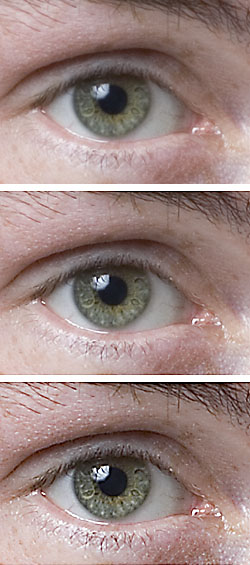
\includegraphics[scale=1.2]{images/unsharpMaskExample.jpg}
\caption{Unsharp mask example. \\
Source: http://upload.wikimedia.org/wikipedia/commons/4/43/Unsharped\_eye.jpg}
\label{unsharpMaskExample}
\end{center}
\end{figure}

\section{Image segmentation}

According to \cite{digitalImageProcessing}, segmentation algorithms partition images into
constituent parts or objects. They are generally based on two basic properties of intensity values:
discontinuity and similarity. In the first case, the approach is to partition an image based on
abrupt changes in intensity (like for example edges in an image). In the second case, the approach is
based on partitioning an image into regions, that are similar (for example they have similar color).
There are many segmentation algorithms available. Solution presented in this work is based on
thresholding approach.

\subsection{Tresholding}

Thresholding, thanks to its properties and simple implementation, is one of the most commonly used
segmentation algorithms. In the most basic form, having gray level of each pixel in an image it is
possible to find a value of threshold, which will separate groups with different gray-level values.
Then the appropriate, different color value for pixels, which are above and below threshold value
is set.

Let's assume, that:
\begin{itemize}
  \item T is a threshold value
  \item f(x, y) is a gray-level value in a point x, y
  \item g(x, y) is a thresholded pixel value
\end{itemize}

$$
g(x, y) = \left\{ \begin{array}{ll}
1 & \textrm{if $f(x, y) \geq T$}\\
0 & \textrm{if $f(x, y) < T$}\\
\end{array} \right.
$$

Algorithm takes one parameter - T, which is a thresholding value.

Example image with applied thresholding ( with T = 130 ) is presented in a 
Fig.~\ref{thresholdingExample}.

\begin{figure}[ht]
\begin{center}
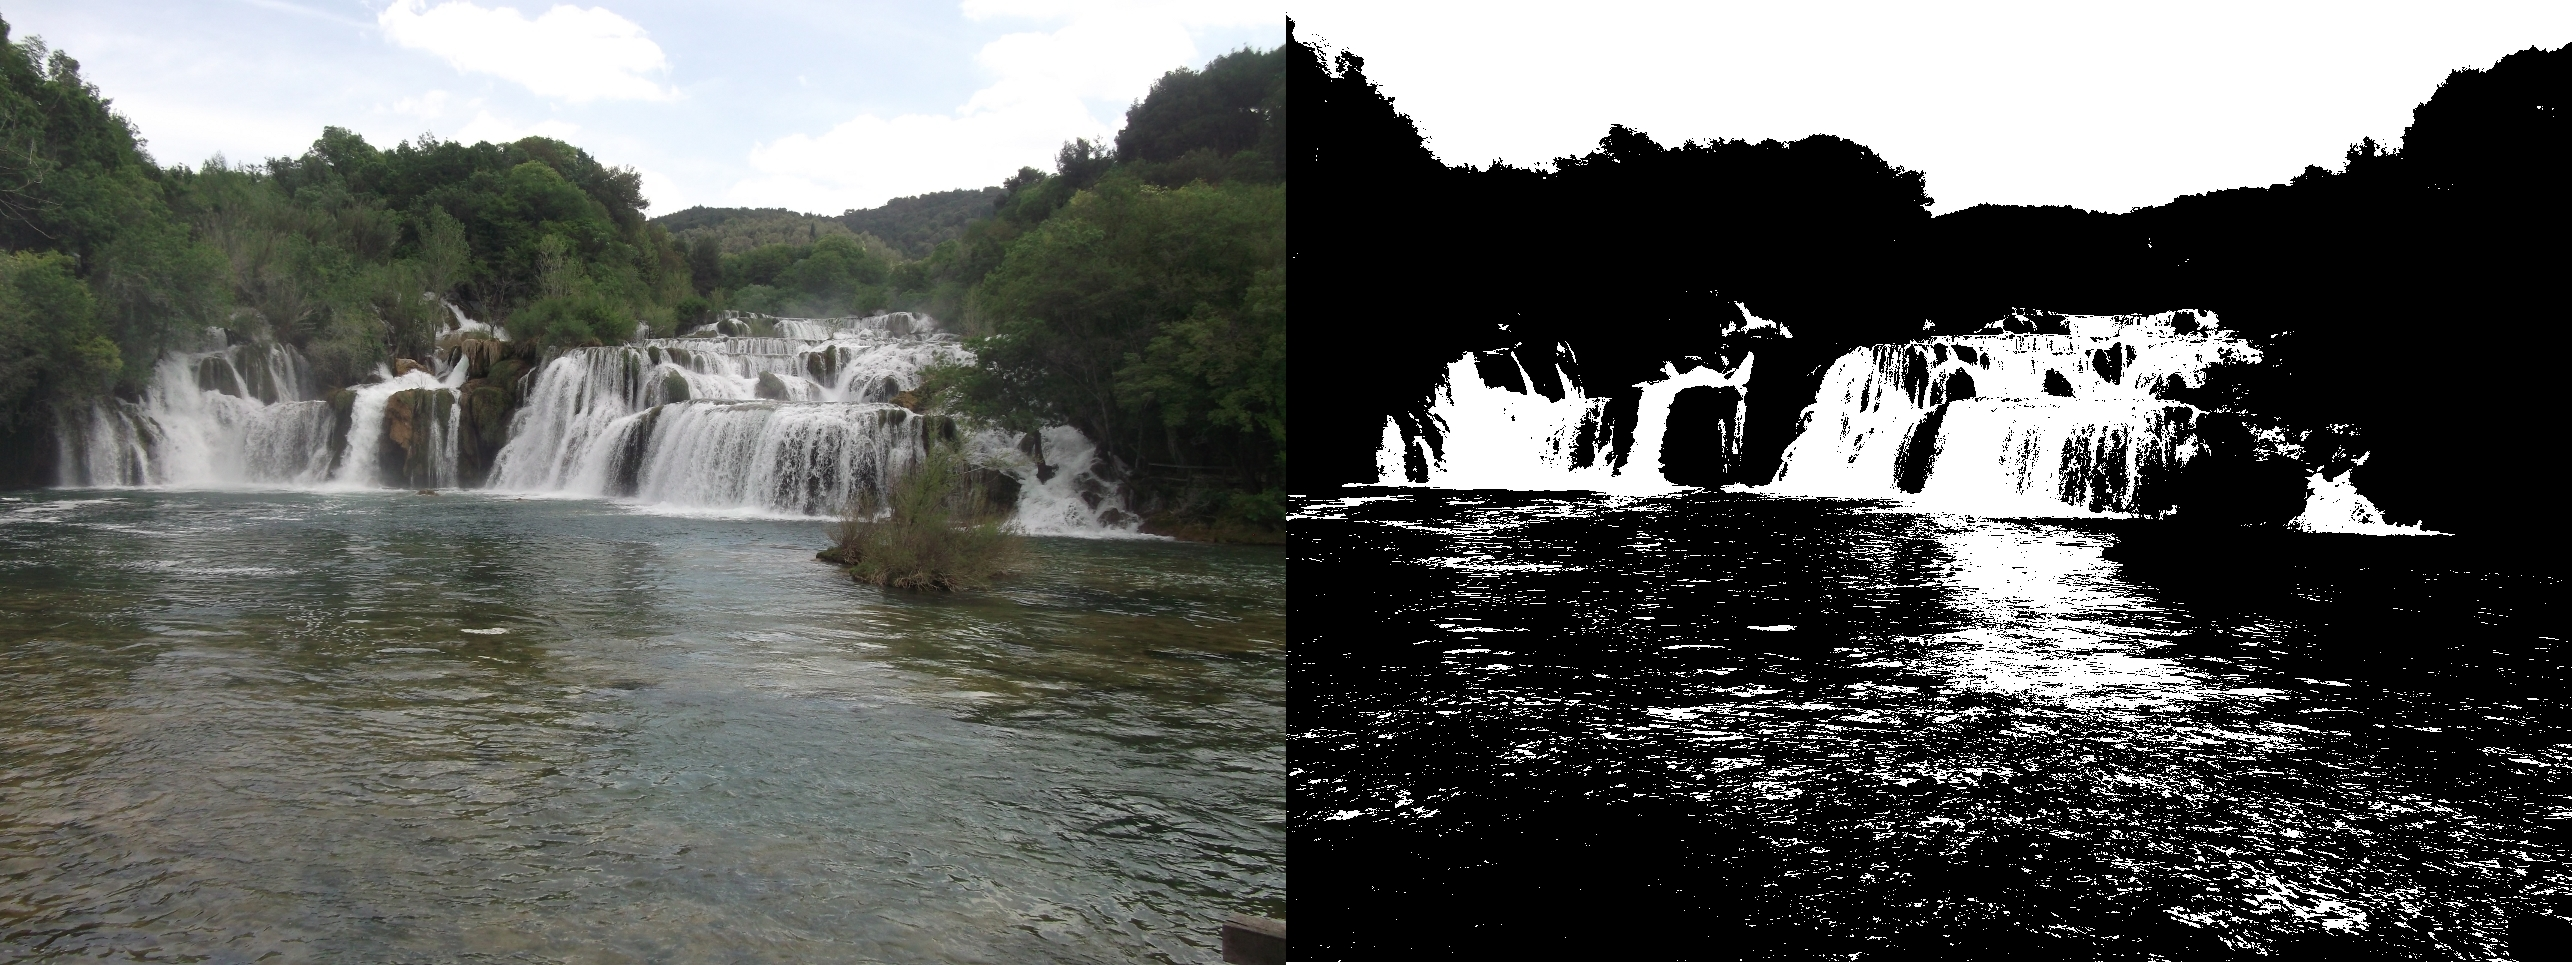
\includegraphics[scale=0.15]{images/thresholdingExample.jpg}
\caption{Thresholding example. \\
Source: own}
\label{thresholdingExample}
\end{center}
\end{figure}

\subsection{Principles of grouping}

According to \cite{gestaltTheory}, the Principles of Grouping (known also as Gestalt laws or
grouping) starts with the assumption of active grouping laws in visual perception. These groups are
identifiable with subsets of the retina. Whenever points (or previously formed groups) have one or
several characteristics in common, they get grouped and form a new larger visual object. Gestalt
basic grouping principles are:

\begin{description}
  \item[Vicinity] for example pixels glued together or objects which are close enough to each other
        and apart enough from the rest to build a group;
  \item[Similarity] for example similarity of color, shape, texture, orientation;
  \item[Continuity of direction] which for example can be applied to an array of objects;
  \item[Constant width] which is very relevant for drawings and all kinds of natural and artificial
        forms;
  \item[Convexity] which applies to closure and continuation of objects;
  \item[Past Experience] which applies, when some generic shapes can be interpreted as familiar
        objects(for example an oval interpreted as a face).
\end{description}

\section{Color image printing}

According to \cite{cmykWiki} and \cite{halftoneWiki}, color images are printed using a CMYK (Cyan,
Magenta, Yellow and Key - Black) model. The final printing color using a CMYK model is achieved by
linking of each basic color in a proportion from 0\% to 100\%. Individual color layers are linked by 
overlapping (not mixing). In a CMYK printing halftone method is used. It is a reprographic technique
that simulates continuous tone imagery through the use of dots, varying either in size, in shape or
in spacing, thus generating a gradient like effect. Where continuous tone imagery contains an
infinite range of colors or greys, the halftone process reduces visual reproductions to an image
that is printed with only one color of ink, in dots of differing size. To improve image quality, the
screen for each color is set at a different angle. Without halftoning, the three primary process
colors could be printed only as solid blocks of color, and therefore could produce only seven
colors. With halftoning, a full continuous range of colors can be produced.

\section{Color image scanning}

According to \cite{imageScanner}, image scanner is a device, that optically scans images and
converts them to digital ones. The most commonly used type is called flatbed scanner. It is composed
of a glass pane on which document is placed to be scanned. Typical modern scanners use a 
charge-coupled device (CCD) or Contact Image Sensor (CIS) as the image sensor. In case of CCD, under
the glass pane there is a bright light, which illuminates it and a moving three optical arrays of
sensors with red, green and blue filters. CIS scanners consist of moving set of LEDs strobed for
illumination and a connected monochromatic photodiode array under a rod lens array for light
collection.

The scanned result is a raster image - a dot matrix data structure representing a generally
rectangular grid of pixels, or points of color, stored in a memory as an image file in a varying
formats. Unfortunately resulting raster image has many false colors caused by for example an RGB
misalignment (described widely in \cite{colorMapSegmentation}).

\section{Color scanned maps processing}

Processing of color scanned maps is a very interesting topic. There are some research works focusing
on it. In this section there are short descriptions of found six algorithms, which focus on this
problem. \\

In \cite{semanticAnalysisAndRecognition}, authors treat alphanumerical signs, letters, points, lines
and areas separately. Image is vectorized and segmented in separate processes. To separate 
alphanumerical characters, there is used a \textit{False Color Technique}. Next, the 
\textit{Composite Image Technique} is used to decompose image and link objects by their associated
names. Finally, set of separate modules grouped as \textit{A2R2V} detect alphanumeric, punctual and
linear characters in the map. In this algorithm there are used such techniques like thresholding,
color segmentation and neural networks. \\

Another approach is presented in \cite{comparativeAnalysisOfScannedMaps}. This work focused on 
decomposition of scanned topographic maps. Algorithm finds different areas (like lakes, rivers,
contours, text, grid and other) using map analysis and thresholding in a black and white mode.
Next, there are used filtering algorithms to remove elements smaller than expected and noise.
Then map texture is analysed. This step is helpful in detection of areas like for example lakes.
Algorithm uses thresholding, median filter and many color segmentation techniques. \\

Next method is shown in \cite{colorsOfThePast}. Authors of this research worked with maps from 
19th century. The algorithm is divided into four stages. First, the clustering algorithm allows 
automatic determination of the pixels, which represent color layer prototypes in three domains:
local image domain, histogram analysis and color space. In the second phase, pixels are defined as
layer specific seeds based on distances in color space to the color points of the computed layer 
prototypes and local homogenity. The third phase takes the result of previous part and identifies 
connected regions of pixels belonging to one of the color layers. Finally, unallocated pixels are
joined to nearest groups. \\

Another solution is presented in \cite{automaticVectorization}. This work is focused on segmentation
of contour maps. There are used \textit{Deformable Model Tracking} and \textit{Adaptive Flow 
Orientation}. It uses a seed segment searching and variable force control. Contour lines are 
detected automatically. This method is good at detection of crossed, broken and touching lines. \\

Next algorithm can be found in \cite{topographicMapsAutomaticVectorization}. In this work image is
segmented with a "Peeling Onion Strategy". Layers are recognized separately. Each recognized layer
is subtracted of the map to facilitate the interpretation of remaining, more complex ones. Sequence
of processes is as follows:

\begin{itemize}
  \item Recognition of objects for which there is an external data available;
  \item Recognition and vectorization of textured areas;
  \item Recognition of strings and symbols;
  \item Recognition of objects with variable shape;
  \item Recognition of networks.
\end{itemize}

In these processes there are used: pattern matching, contour following, polygonal approximation and
skeletonization algorithms.

Last presented approach is shown in \cite{colorMapSegmentation}. There is presented a segmentation
method dedicated for United States Geological Survey (U.S.G.S.) topographic maps. Algorithm first 
segments out white background. Next, image is segmented using Eigenvector line fitting technique.
Algorithm knows typical values of colors used in U.S.G.S. In the final part of the algorithm, proper
color value is set for every pixel (it is based on distance of pixel Eigenvector and Eigenvalue and
a known value from U.S.G.S. colors standard). Summarizing, the segmentation algorithm uses knowledge
about colors used in maps from U.S.G.S.

\chapter{Research of the topic}

This chapter focuses on a description of the input data and problems related to the segmentation
process discovered during research of the topic.

\section{Input data description}

Algorithm input is a color-scanned map saved on the disk as a digital image. Its resolution is
arbitrary. Example image is presented in a Fig.~\ref{inputExample}. It is a scanned color map of a
Polish city - Brzeg.

\begin{figure}[!ht]
\begin{center}
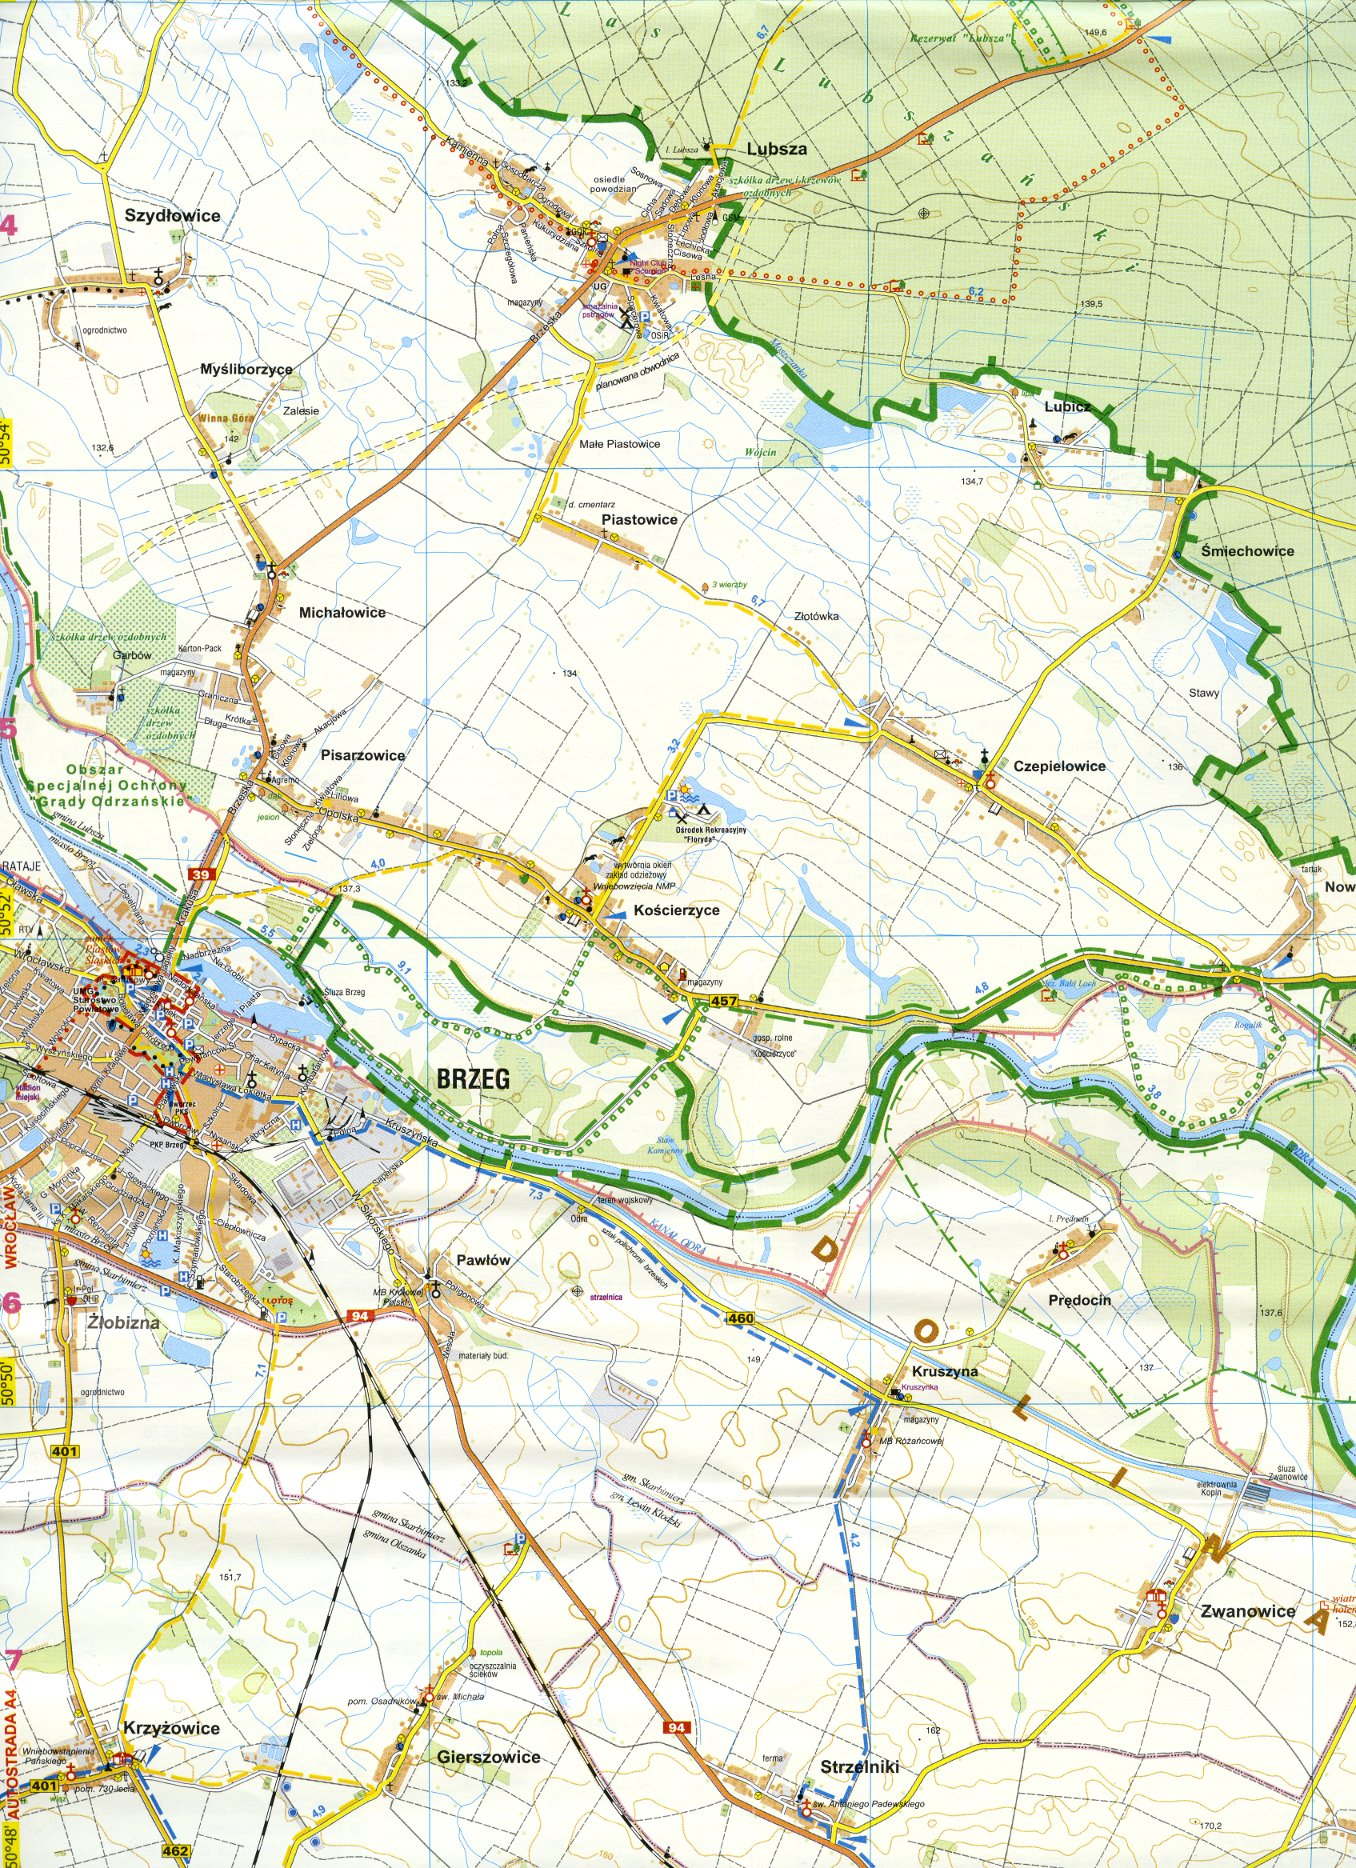
\includegraphics[scale=0.78]{images/brzeg.jpg}
\caption{Example input.}
\label{inputExample}
\end{center}
\end{figure}

\section{Problems and restrictions}

There are a lot of problems associated with segmentation of scanned maps. Due to imperfection of
a scanning process, resulting color scanned digital images have many distortions. There are also
problems connected with input images (they can be damaged before scanning). Moreover, raster derived
from printed document should be removed. Additionaly maps have many small elements and text. These
details, as well as shape of background areas (like for example lakes and forests) should be kept in
resulting image. All found problems are described more precisely in next sections.

\subsection{Input image and scanning process quality}

Scanned digital images have many distortions. They are related to the damage of an input image, like
places, where maps are creased (example in Fig.~\ref{creaseExample}) or dirty (shown in a 
Fig.~\ref{dirtyExample}). It results in the existence of darker elements in the output image.

\begin{figure}[!ht]
\begin{center}
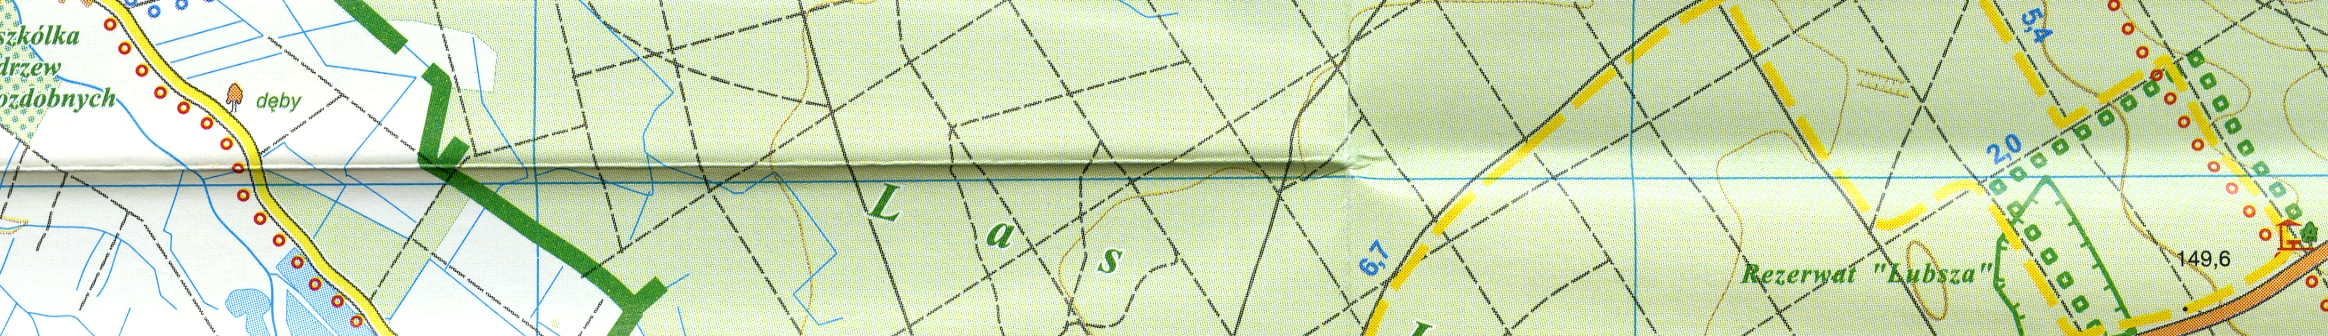
\includegraphics[scale=1.1]{images/creaseExample.jpg}
\caption{Example of distortion caused by creased maps.}
\label{creaseExample}
\end{center}
\end{figure}

\begin{figure}[!ht]
\begin{center}
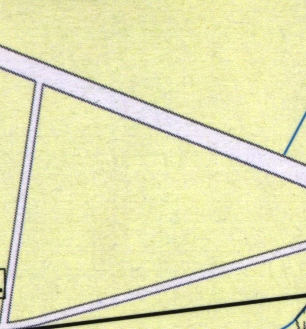
\includegraphics[scale=3.0]{images/dirtyExample.jpg}
\caption{Example of distortion caused by dirty map.}
\label{dirtyExample}
\end{center}
\end{figure}

Another problems are related to scanning process. Resulting images are noisy. Additionaly a
scanning device or scanned map can be dusty. These problems result in small distortions, which
should not be placed in an output image. Example of this situation is presented in a 
Fig.~\ref{dustExample}. It is marked in the red rectangle.

\begin{figure}[!ht]
\begin{center}
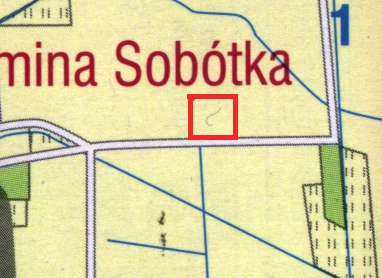
\includegraphics[scale=3.0]{images/dustExample.jpg}
\caption{Example of distortion caused by dust.}
\label{dustExample}
\end{center}
\end{figure}

Next problem is related to the double-sided printing of the map. It is sometimes a problem, because
in some cases second side of the map is visible in a scanned image. This situation is presented in a
Fig.~\ref{doubleSidedMap}.

\begin{figure}[!ht]
\begin{center}
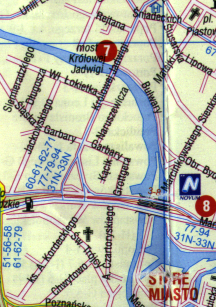
\includegraphics[scale=0.8]{images/doubleSidedMap.png}
\caption{Example of distortion caused by visible second side of the map.}
\label{doubleSidedMap}
\end{center}
\end{figure}

Finally, resulting image can have undesirable areas with wrong (usually darker) color. Their
existence is caused by mistakes made during scanning process, for example when image is not properly
put in a scanner surface. This situation is visualized in a Fig.~\ref{badScanExample}.

\begin{figure}[!ht]
\begin{center}
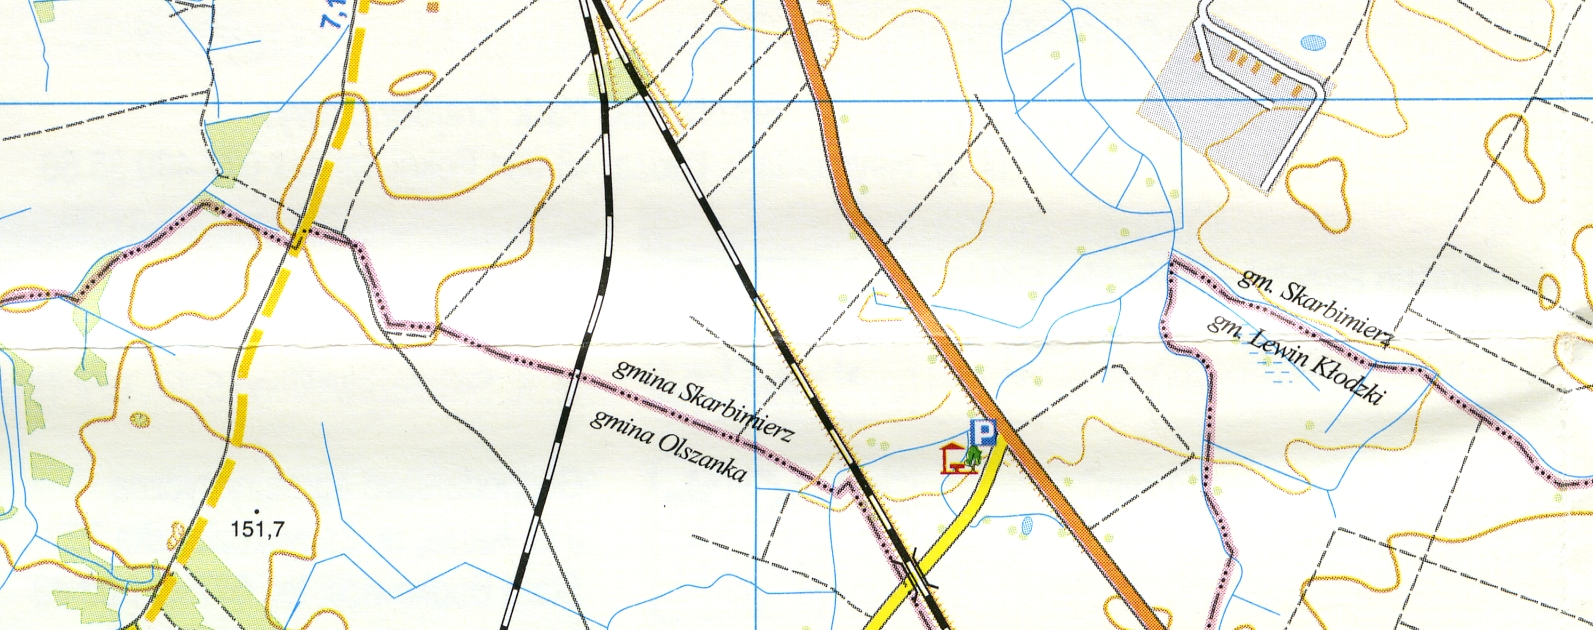
\includegraphics[scale=1.3]{images/badScanExample.jpg}
\caption{Example of distortion caused by improper scanning.}
\label{badScanExample}
\end{center}
\end{figure}

\subsection{Small details}

Input image contains many small details. They exist especially in city and topographic maps.
City maps contain a lot of small elements, like churches, parking places or gas stations.
Additionaly, in cities there are many roads and areas, which are marked in different colors. 
Furthermore they contain many small letters, which, for example, indicate names of streets, parks
or major buildings and places. Finally, in the city map, lines, roads and test are often crossing
each other. Example fragment of a city map is shown in a Fig.~\ref{cityExample}.

\begin{figure}[!ht]
\begin{center}
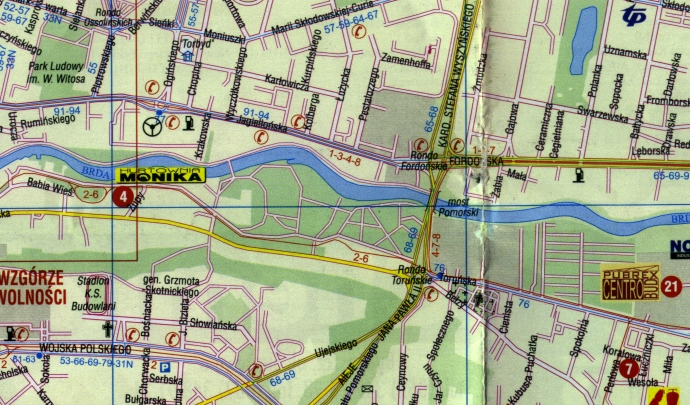
\includegraphics[scale=0.65]{images/cityExample.jpg}
\caption{Fragment of a city map.}
\label{cityExample}
\end{center}
\end{figure}

Another problems are related to topographic maps. They have small letters and elements in different
colors. Additionaly they contain very thin topographic lines. Many of them are not continuous
 (some lines are even marked as dots in the same color). These problems are shown in a fragment of a
topographic map in a Fig.~\ref{topographicMapExample}.

\begin{figure}[!ht]
\begin{center}
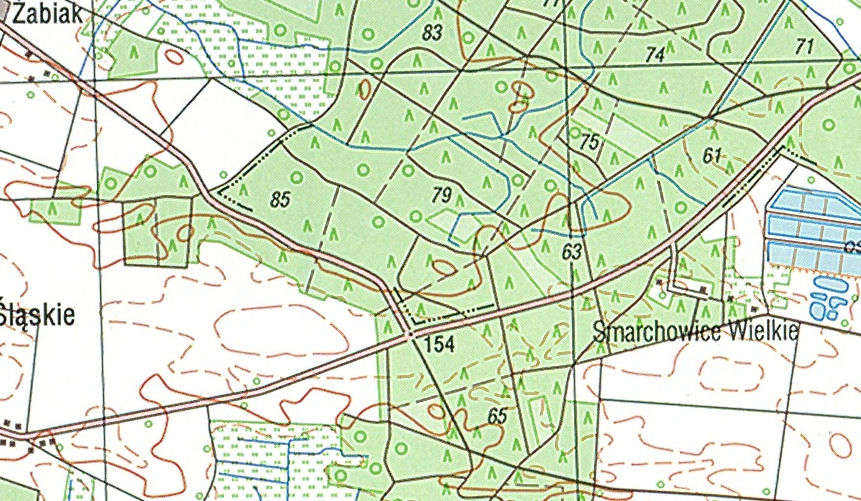
\includegraphics[scale=2.0]{images/topographicMapExample.jpg}
\caption{Fragment of a topographic map.}
\label{topographicMapExample}
\end{center}
\end{figure}

\subsection{Raster elimination}

Digital image coming from a scanner is a raster image. Every pixel is defined itself. This
representation has some disadvantages. One of them is called moro effect. It interferes with
segmentation algorithm. Example of a moro effect is shown in a Fig.~\ref{moroEffectExample}

\begin{figure}[!ht]
\begin{center}
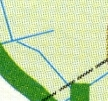
\includegraphics[scale=11.0]{images/moroEffectExample.jpg}
\caption{Example of a moro effect.}
\label{moroEffectExample}
\end{center}
\end{figure}

\chapter{Design of the algorithm}

In this chapter there is a full description of an algorithm processing scanned maps.

\section{Main parts of the algorithm}

Map segmentation is a complicated process. In the one hand, all background should be segmented with
as small number of mistakes as possible. To reduce scanning errors and unify background, many 
smoothing algorithms can be applied, like for example Gaussian Filter. On the other hand there is a
lot of details, lines and text like for example streets, toponyms, symbols and topographic lines.
In this case using smoothing algorithms with bigger parameter values is not a good idea - these
algorithms cause, that for example text is deformed and is not as sharp as in the input image. To
solve these problems, algorithm has been divided into two parts. First one is responsible for
detection of all details (roads, text, lines, rivers). Second one detects background of the map. Both
algorithms work independently and take as an input the same, image. They can work simultaneously.
Results of segmentation of both layers are merged to one output image. Flow of the algorithm is
presented on a statechart in a Fig.~\ref{algorithmParts}.

\begin{figure}[!ht]
\begin{center}
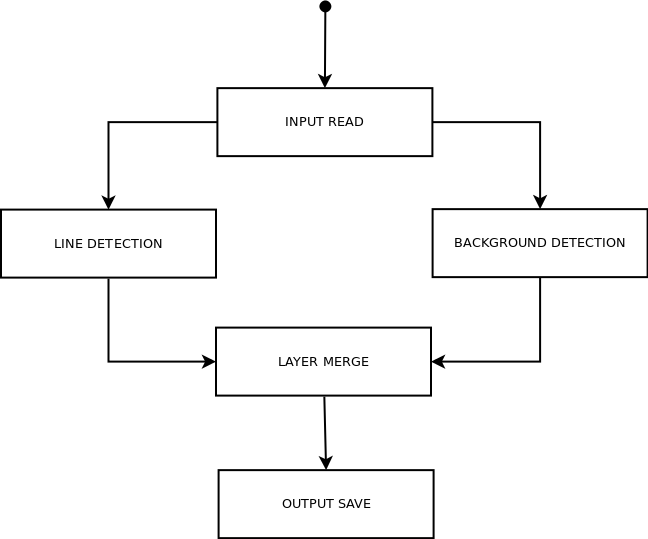
\includegraphics[scale=0.5]{images/allAlgorithmParts.png}
\caption{Parts of the algorithm.}
\label{algorithmParts}
\end{center}
\end{figure}

\section{Detection of areas}

The main aim of this part is to detect all background elements, like for example lakes, forests and
thicker lines (rivers, main roads). The algorithm focuses on elimination of all distortions and on
detection and unification of areas. This method should remove all thiner lines and small details
from an image. In an output image there should appear all background elements. Every separate
area should have a different color. Main distortions should be eliminated.

\subsection{Algorithm parts}

The algorithm firstly applies a group of algorithms to remove some distortions and prepare image for
a final segmentation. In this case there are used some smoothing algorithms, like Gaussian Filter
and Bilateral Filter. Then, smaller details are eliminated. To do that, there are used Dilation and
Erosion algorithms. In the next step image is segmented. Main aim of this part is to unify color of
each area. Finally, the smallest areas are eliminated from an output image. They are substituted
with colors of areas, which are around them. Flow of the background detection algorithm is presented
in a Fig.~\ref{backgroundDetectionImage}

\begin{figure}[!ht]
\begin{center}
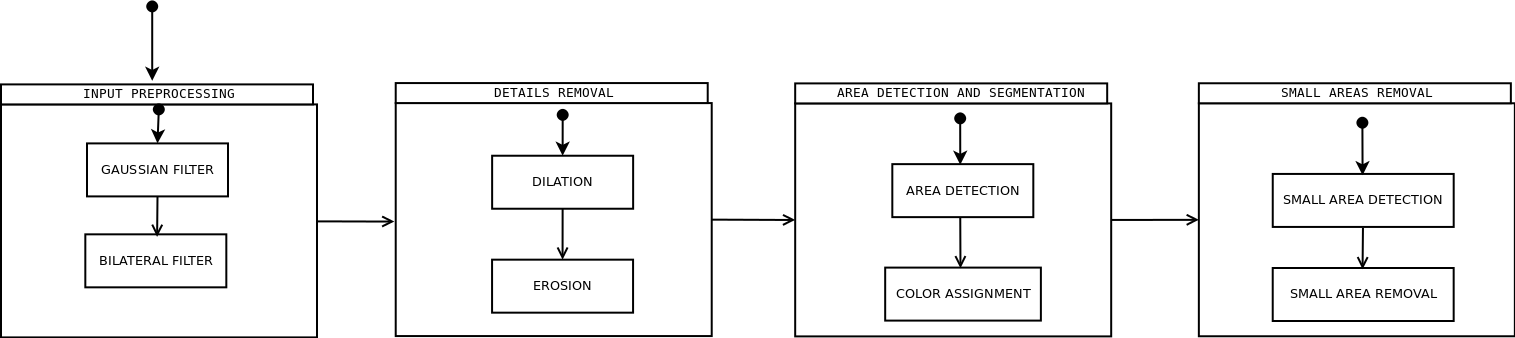
\includegraphics[scale=0.3]{images/backgroundDetection.png}
\caption{Background detection process.}
\label{backgroundDetectionImage}
\end{center}
\end{figure}

\subsubsection{Input preprocessing}

In an input preprocessing part there were used two algorithms: \textit{Gaussian Filter} and \textit{
Bilateral Filter}. Usage of first one is a very good method in elimination of raster and small
distortions (like for example dust). The procedure is applied with a big value of \textit{Radius}
parameter - it helps to remove more distortions. It causes loss of image sharpness, but it is
irrelevant in this case. In a Fig.~\ref{gaussianBlurResult} there is an example usage of a Gaussian
Filter with \textit{Radius} = 5. All major distortions and moro effect do not exist in a resulting
image. Sharpness of the text (in this case name of the river) is lost.

\begin{figure}[!ht]
\begin{center}
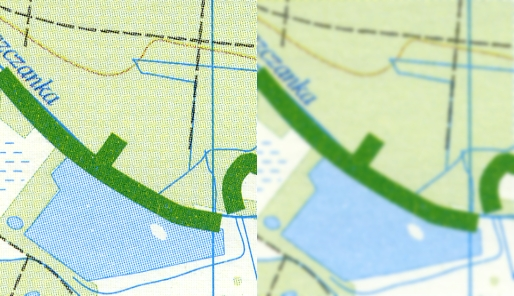
\includegraphics[scale=3.0]{images/GaussianBlurResult.jpg}
\caption{Fragment of a map of Brzeg with Gaussian Blur with Radius = 5 applied. \\ 
Original image is on the left. On the right side there is a resulting image.}
\label{gaussianBlurResult}
\end{center}
\end{figure}

Second algorithm - bilateral filter reduces noise, which was visible in an input map. It has also
another advantage - all edges are kept. In case of the background detection, similarly to Gaussian
Filter, large values of parameters are used. It causes, that a bilateral filter has a big influence
on the resulting image. Colors of all areas are aligned. In a Fig.~\ref{bilateralFilterResult},
there is an example result of applying bilateral filter. Colors of green areas, border line, roads
and a town are aligned. Some small details dissapeared.

\begin{figure}[!ht]
\begin{center}
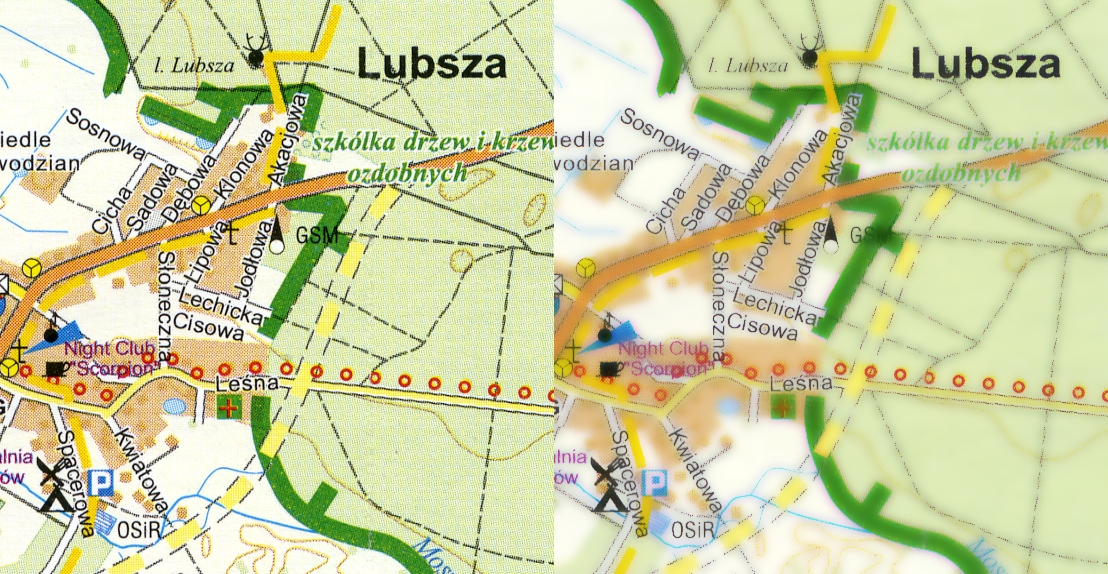
\includegraphics[scale=1.5]{images/BilateralFilterResult.jpg}
\caption{Fragment of a map of Brzeg with Bilateral Filter with Diameter = 30 and Delta values = 150
applied. Original image is on the left. On the right side there is a resulting image.}
\label{bilateralFilterResult}
\end{center}
\end{figure}

\subsubsection{Removal of details}

Erosion and Dilation algorithms are useful in removing noise, joining or isolation of individual
elements and finding intensity holes or bumps in an image. Thanks to these properties, it is easy
to eliminate unwanted, small elements from an image like roads, rivers, small details (in cities) or
topographic lines. These algorithms are helpful in removal of some distortions of a map, like for
example darker areas caused by unproper scanning process or map creases - image after application of
these algorithms have these unwanted areas eliminated. Usage of dilation cause, that all thin areas
dissapear. Furthermore, distance between every separate element grows.

\begin{figure}[!ht]
\begin{center}
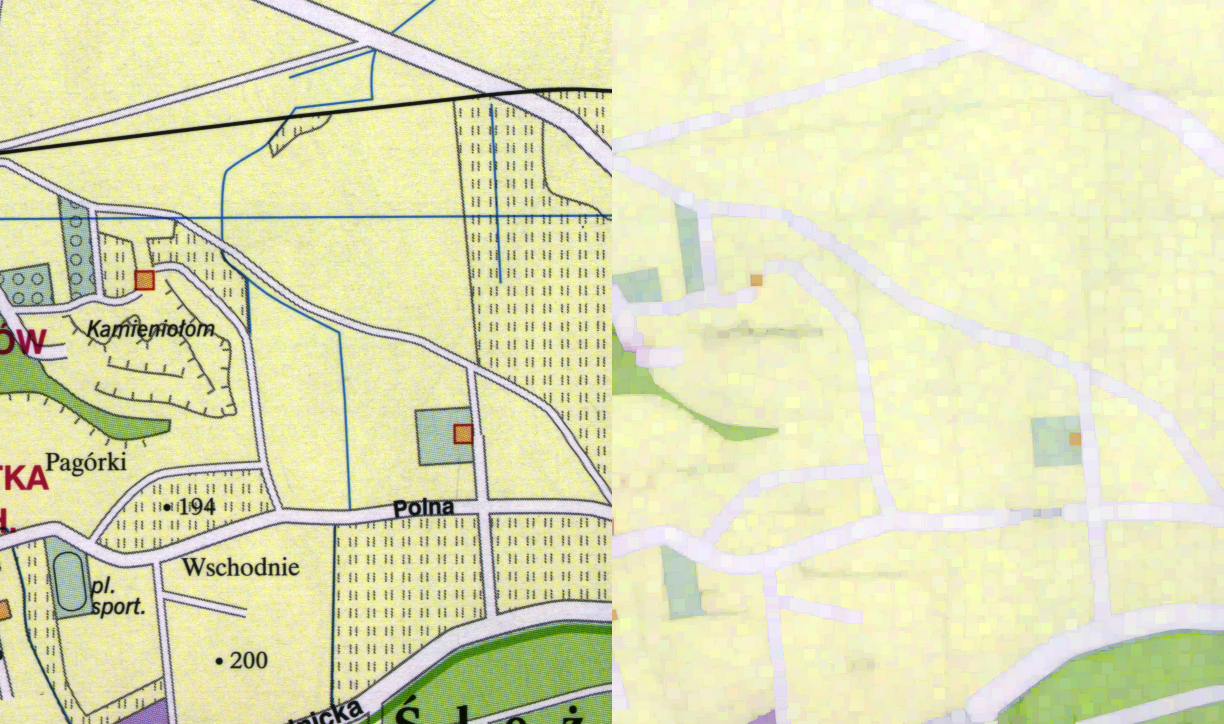
\includegraphics[scale=1.0]{images/dilationResult.png}
\caption{Fragment of a map of Sobótka with dilation applied (5 times). \\
Original image is on the left. On the right side there is a resulting image.}
\label{dilationResult}
\end{center}
\end{figure}

Example of dilation usage is in a Fig.~\ref{dilationResult}. All thin lines are eliminated from the
resulting image. In the output there are visible only yellow and green background elements (with some
distortions eliminated). Moreover there is a background of roads and areas of three smaller elements.

Erosion does the opposite - it causes, that all lines become thicker. It also merges broken
elements. Example of its use is in a Fig.~\ref{erosionResult}. Every line is thicker than in the
original. Borders of every area are easy to determine. Colors of areas are darker and unified.

\begin{figure}[!ht]
\begin{center}
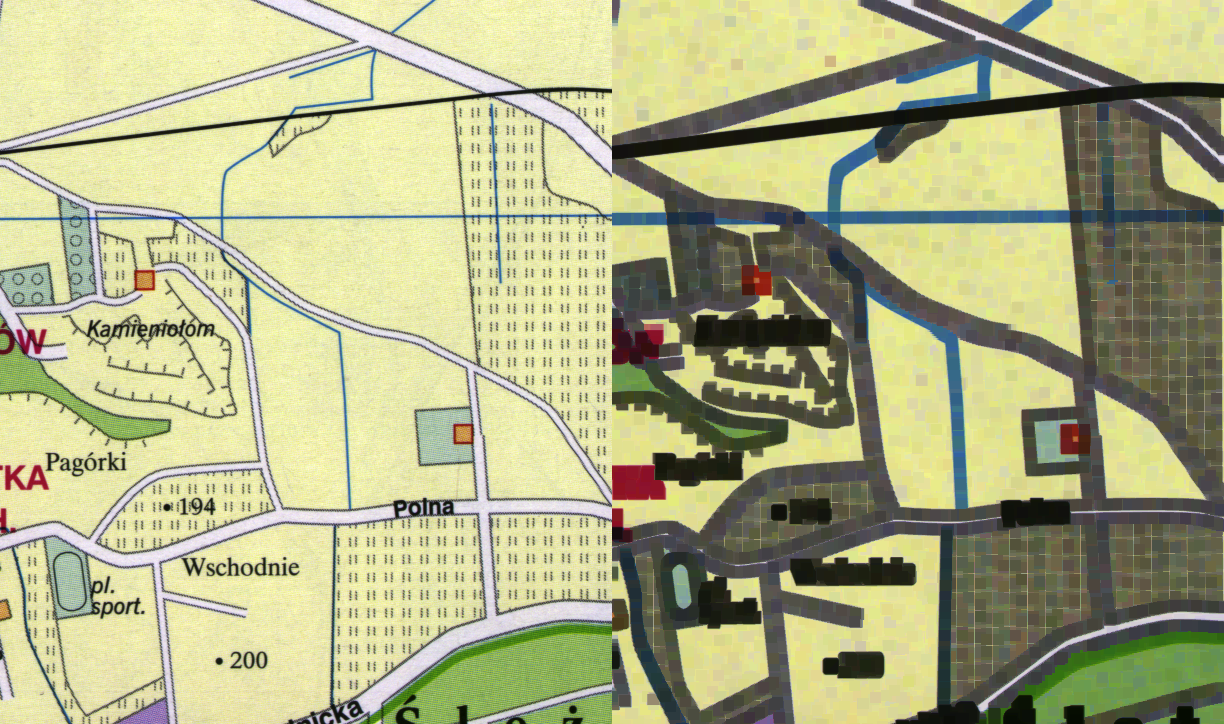
\includegraphics[scale=1.0]{images/erosionResult.png}
\caption{Fragment of a map of Sobótka with erosion applied (5 times). Original image is on the left.
On the right side there is a resulting image.}
\label{erosionResult}
\end{center}
\end{figure}

In case of background detection in scanned color maps, these algorithms give the best results when
they are combined together. After applying these operations, noise and all smaller elements (listed
above) are removed. Major distortions are also eliminated. Moreover colors of every area is almost
the same. As a result, these algorithms are an excellent base for segmentation methods. Example
usage of combined dilation and erosion is presented in a Fig.~\ref{dilationErosionResult}. Every
area has different color and output image have unnecessary details eliminated.

\begin{figure}[!ht]
\begin{center}
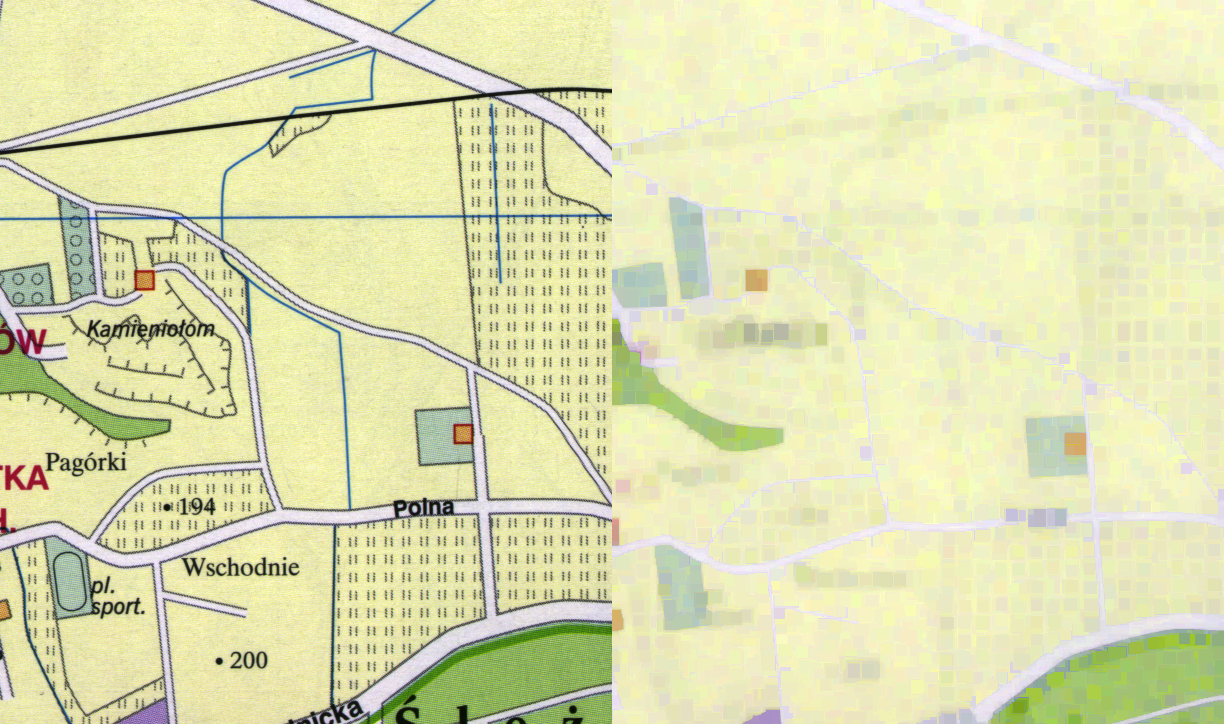
\includegraphics[scale=1.0]{images/dilationErosionResult.png}
\caption{Fragment of a map of Sobótka with dilation (5 times) and then erosion (also 5 times) applied.
Original image is on the left. On the right side there is a resulting image.}
\label{dilationErosionResult}
\end{center}
\end{figure}

\subsubsection{Areas detection and segmentation}

Detection of all map areas is based on two properties. First one is color of every group represented
by their pixels. Second one is a desired number of areas, which should be detected (this number is
easy to determine in case of digital maps). The algorithm at the beggining analyses image pixels and
groups them. As a result there are groups of pixels with a similar color. In the next step,
all groups, which represent similar values are merged until the desired number of colors is reached.
In the last part, each pixel of an image is assigned to best-fitting group. The whole process with
its parameters is described in Algorithms~\ref{colorGroupingAlgorithm},~\ref{groupsMergingAlgorithm}
~and~\ref{colorAssignmentAlgorithm}. \\

Parameters of the algorithm:
\begin{itemize}
  \item \textit{Threshold} - The maximum distance between the currently checked color and a group,
          determining if the color should be assigned into the group
  \item \textit{Maximum Number of Colors}, which determines, how much groups should exist in an
          output map (the actual number of background colors in a map)
\end{itemize}

\begin{algorithm}[!ht]
  \KwData{Threshold}
  \KwIn{Image}
  \KwOut{Colors grouped by color similarity}

  GroupContainer gc\;
  \ForEach{Pixel in Image}
  {
    pixelAddedToGroup := false\;
    \ForEach{Group in gc}
    {
      \If{distance(Pixel.color, Group.averageColor) < Threshold}
      {
        Group.add(Pixel)\;
        pixelAddedToGroup := true;
      }
    }

    \If{pixelAddedToGroup = false}
    {
      gc.createNewGroup(Pixel)\;
    }
  }

  \Return{gc}

  \caption{Color grouping}
  \label{colorGroupingAlgorithm}
\end{algorithm}

\begin{algorithm}[!ht]
  \KwData{Threshold}
  \KwData{MaximumNumberOfColors}
  \KwIn{GroupContainer gc}
  \KwOut{SegmentedImage}

  \Repeat{gc.numberOfGroups > MaximumNumberOfColors}
  {
    \ForEach{Group in gc}
    {
      \ForEach{AnotherGroup in gc}
      {
        \If{distance(Group.averageColor, AnotherGroup.averageColor) < Threshold)}
        {
          merge(Group, AnotherGroup)\;
        }
      }
    }
    Threshold := Threshold + 1\;
  }

  \Return{gc}

  \caption{Groups merging}
  \label{groupsMergingAlgorithm}
\end{algorithm}

\begin{algorithm}[!ht]
  \KwIn{GroupContainer gc}
  \KwIn{Image}
  \KwOut{SegmentedImage}

  \ForEach{Pixel in Image}
  {
    group := gc.getBestFittingGroup{Pixel}\;
    Pixel.color := group.averageColor\;
  }

  \Return{Image}

  \caption{Color assignment}
  \label{colorAssignmentAlgorithm}
\end{algorithm}

The distance between colors is Euclidean:~
$$
distance(c1, c2) = \sqrt{(c1.red - c2.red)^2 + (c1.green - c2.green)^2 + (c1.blue - c2.blue)^2}
$$

The color of entire group is counted as average value of red, green and blue of every pixel
belonging to this group. The best fitting group for a pixel is that one, which distance to the pixel
is the smallest.

\begin{figure}[!ht]
\begin{center}
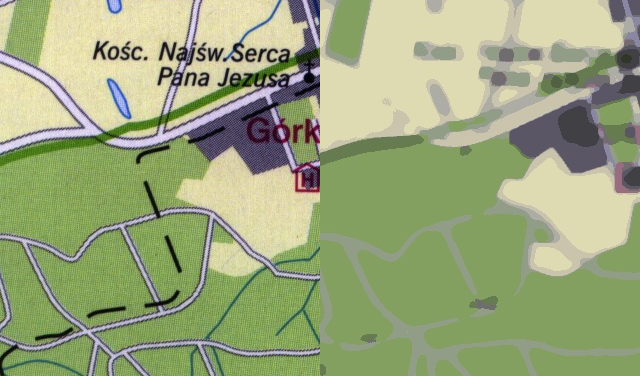
\includegraphics[scale=2.5]{images/segmentationResult.png}
\caption{Fragment of a map of Ślęża with segmentation algorithm applied.
Original image is on the left. On the right side there is a resulting image.}
\label{segmentationResult}
\end{center}
\end{figure}

In a Fig.~\ref{segmentationResult}, there is an example result of applying the segmentation
algorithm. There was used preprocessed (with filtration, dilation and erosion) map of Ślęża. Initial
threshold was set to 30, maximum number of colors was set to 20. Each area has its unified color.
Shape of every area is fairly kept. There are some small areas, which have assigned wrong color.
They exist mainly in places, where there was text in the input image.

\subsubsection{Removal of small areas}

After segmentation of areas in the map, there are often some pixels, which were interpreted as a
wrong area. It is easy to detect this situation, because wrongly assigned pixels are in most of
cases surrounded by properly evaluated elements. To remove such misinterpreted pixels, the Holes
Removal algorithm has been designed. This method investigates surrounding of each pixel in an image.
New color of the pixel is set to the value, which is the most frequent in the surrounding area.
Algorithm has one parameter - it is a size of the matrix, which surrounds the pixel. This matrix is
used for the analysis of color of area, which is around processed pixel. The bigger value is set,
the bigger area is taken into consideration. For example, for parameter value = 7, the surrounding
area is a matrix with a size 7x7. Pseudocode of the algorithm is presented in the Algorithm~
\ref{holesRemovalAlgorithm}.

\begin{algorithm}[!ht]
  \KwIn{WindowWidth}
  \KwIn{Image}
  \KwOut{SegmentedImage}

  \ForEach{Pixel in Image}
  {
    window := getWindow(windowWidth)\;
    newColor := window.getMostFrequentColor\;
    pixel.color := newColor\;
  }

  \Return{Image}

  \caption{Holes removal}
  \label{holesRemovalAlgorithm}
\end{algorithm}

In a Fig.~\ref{holeRemovalResult}, there is preseted example usage of Holes Removal algorithm. It
was applied to previously segmented map of Ślęża. Solution has been applied with a Window Width
parameter set to a very big value - 50. The resulting image has all distortions eliminated.
Unfortunately proper edges and sizes of areas have been lost. It follows, that used window width
parameter value was too big. For bigger values of Window Width argument it is more probable, that
more details will be eliminated and backround borders will be lost.

\begin{figure}[!ht]
\begin{center}
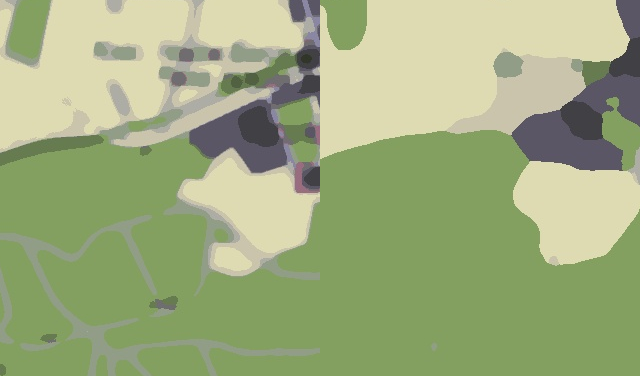
\includegraphics[scale=0.5]{images/holeRemovalResult.png}
\caption{Fragment of a map of Ślęża with Holes Removal algorithm applied.
On the left, there is an image after segmentation. On the right side there is an image with removed
holes.}
\label{holeRemovalResult}
\end{center}
\end{figure}

\subsection{Algorithm parameters}
\label{backgroundDetectionParamsSection}

There are some arguments, which have to be set before application of the algorithm. Their values
depend on the map, to which algorithm is applied. To achieve the best results, every map should have
individually set of parameter values.

\begin{description}
  \item[enabled] \hfill \\
    Determines, if Background Detection algorithm is enabled. \\
    Possible~values:~\{\textit{true},~\textit{false}\};
  \item[gaussian\_blur\_radius] \hfill \\
    Radius of a Gaussian Blur. \\
    Possible~values:~integer number. Proposed~values:~[5~-~15];
  \item[gaussian\_blur\_standard\_deviation] \hfill \\
    Standard deviation of a Gaussian Blur. \\
    Possible~values:~integer number. Proposed~values:~[0~-~5];
  \item[diameter] \hfill \\
    Diameter used by Bilateral Filter. \\
    Possible~values:~integer number. Proposed~values:~[10~-~30];
  \item[sigma\_color] \hfill \\
    Sigma Color used by Bilateral Filter. \\
    Possible~values:~integer number. Proposed~values:~[50~-~150];
  \item[sigma\_space] \hfill \\
    Sigma Space used by Bilateral Filter. \\
    Possible~values:~integer number. Proposed~values:~[50~-~150];
  \item[dilation\_and\_erosion\_size] \hfill \\
    Size of rectangular structuring element used in erosion in dilation algorithms. \\
    Possible~values:~integer number. Proposed~values:~[1-10];
  \item[dilation\_and\_erosion\_counter] \hfill \\
    Number of erosion and dilation applications. \\
    Possible~values:~integer number. Proposed~values:~[2~-~10];
  \item[window\_width] \hfill \\
    Width of a window used by Holes Removal algorithm. \\
    Possible~values:~integer number. Proposed~values:~[5~-~15];
  \item[max\_number\_of\_colors] \hfill \\
    Maximal number of colors, which should be visible in resulting map. \\
    Possible~values:~integer number. Proposed~values:~[10~-~50].
\end{description}

\section{Detection of details}

The main aim of this part of the algorithm is to detect and unify smaller elements, which exist in
the map. These are for example:
\begin{itemize}
  \item thin lines like for example streets, roads, rivers, topographic lines, etc.;
  \item Strings: toponyms and other text, names of the streets;
  \item Small elements from the legend, like for example churches, parking places.
\end{itemize}

The algorithm focuses mainly on filtering out the background, detecting all types of elements and
finally, classification of every detected element or line to one of previously discovered groups.
The result of this part should be an image with isolated and properly classified all map details.

\subsection{Algorithm parts}

In the first step, the algorithm tries to remove all background from the map and keep only small
details. In this case there is a thresholding algorithm used. Next, there is applied a procedure,
which removes all distortions remained in the thresholded image. In this part there is called a 
procedure, which finds and removes all single occuring (lonely) pixels. In the next step, there is
applied an unsharp mask which improves image quality. Finally, all elements are recognized and 
classified to appropriate group. Flow of the entire algorithm is presented in a 
Fig.~\ref{detailDetectionFlow}.

\begin{figure}[!ht]
\begin{center}
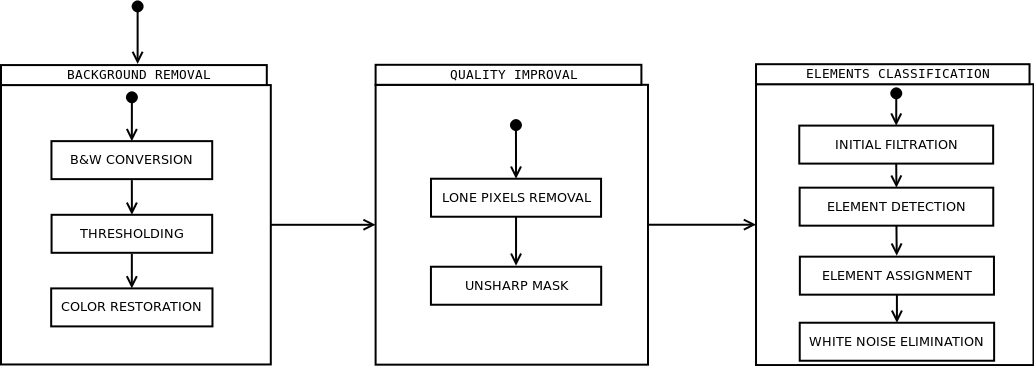
\includegraphics[scale=0.4]{images/detailDetectionFlow.png}
\caption{Flow of the Detail Detection algorithm}
\label{detailDetectionFlow}
\end{center}
\end{figure}

\subsubsection{Background removal}

To remove background from the image, modified thresholding method is used. At the beginning, there
are created three Black and White images. Their pixel values are represented by intensities of red,
green and blue colors. Prepared in this way maps are then thresholded. Values greater than specified
threshold value are marked as a black (Intensity Value = 0), the rest is marked as a white (Intensity
Value = 255). In the next part, three resulting images are merged into one. If any of pixels from
thresholded pixels is black, it is marked in a resulting image. Finally, image colors are restored.
Pixel colors from the original image are assigned for each black pixel from thresholded image.
Pseudocode of the algorithm is presented in Algorithm~\ref{thresholdingAlgorithm}.

\begin{algorithm}[!ht]
  \KwIn{ThresholdValue}
  \KwIn{InputImage}
  \KwOut{ThresholdedImage}

  redIntensity := InputImage.getRedIntensity\;
  greenIntensity := InputImage.getGreenIntensity\;
  blueIntensity := InputImage.getBlueIntensity\;

  threshold(redIntensity)\;
  threshold(greenIntensity)\;
  threshold(blueIntensity)\;

  ThresholdedImage := InputImage\;

  \ForEach{PixelPosition in ThresholdedImage}
  {
    \If{ redIntensity.at(PixelPosition).isWhite() AND greenIntensity.at(PixelPosition).isWhite() AND
         blueIntensity.at(PixelPosition).isWhite() }
    {
      ThresholdedImage.at(PixelPosition).color := WhiteColor\;
    }
  }

  \Return{ThresholdedImage}

  \caption{Background removal}
  \label{thresholdingAlgorithm}
\end{algorithm}

\begin{figure}[!ht]
\begin{center}
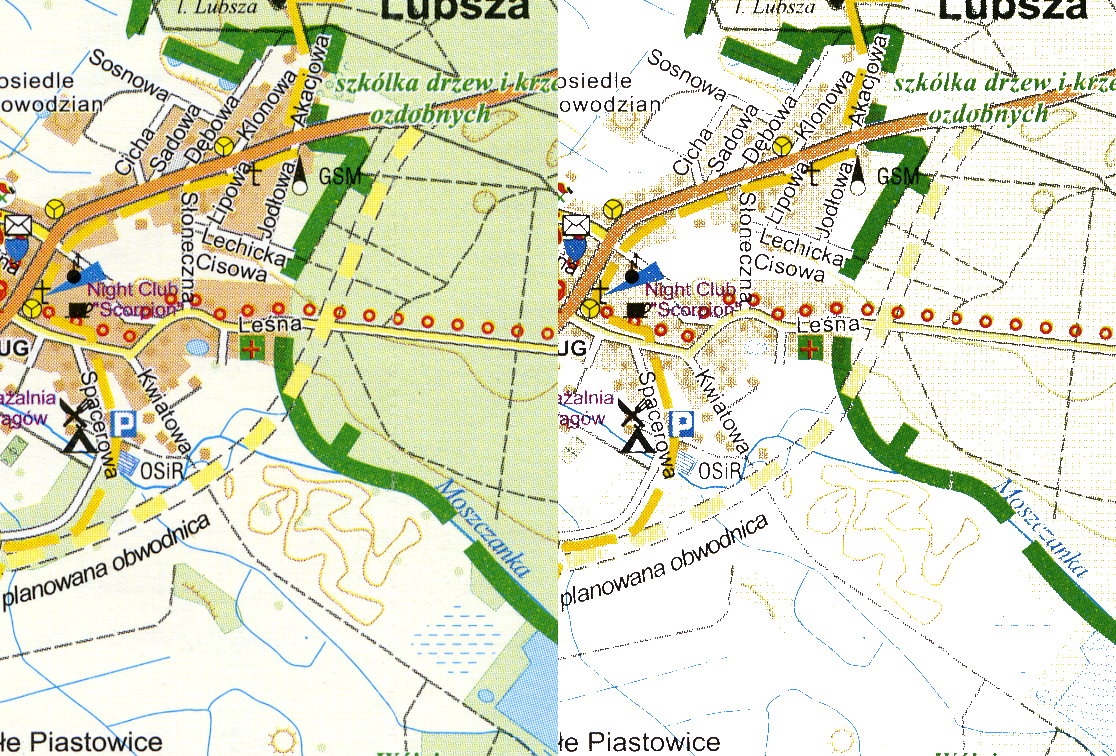
\includegraphics[scale=2.0]{images/thresholdingResult.png}
\caption{Fragment of a map of Brzeg with background detection algorithm applied.
On the left, there is an original image. On the right side there is an image with removed
background.}
\label{thresholdingResult}
\end{center}
\end{figure}

In a Fig.~\ref{thresholdingResult} there is a fragment of a map of Brzeg with removed background.
The background area was removed, but in the output image there are some residues - single dots
visible, especially inside Lubsza town. These errors are very similar to white noise and should be
eliminated in next part of the algorithm.

\subsubsection{Quality improval}

Thresholded image has some background residues. In a resulting image it looks very similar to white
noise. There are many single pixels, which were not eliminated during thresholding process. To
remove these unwanted features, the algorithm of removing lonely pixels is applied. This method
analyses every pixel of an image and removes all colored dots, which surrounding is white.
Additionaly, value of all white pixels, which are surrounded by colored ones is changed to average
of its surrounding pixels values. Pseudocode of the algorithm is presented in
Algorithm~\ref{singleDotsRemovalAlgorithm}.

\begin{algorithm}[!ht]
  \KwIn{ThresholdedImage}
  \KwOut{ProcessedImage}

  ProcessedImage := ThresholdedImage\;

  \ForEach{Pixel in ProcessedImage}
  {
    \eIf{ Pixel.isWhite() }
    {
      \If{ allSurroundingIsColored( Pixel ) }
      {
        Pixel.color := AverageColorOfSurrounding\;
      }
    }
    {
      \If{ allSurroundingIsWhite( Pixel ) }
      {
        Pixel.color := WhiteColor\;
      }
    }
  }

  \Return{ProcessedImage}

  \caption{Single dots removal}
  \label{singleDotsRemovalAlgorithm}
\end{algorithm}

Example of application of removing lonely pixels is presented in a Fig.~\ref{removeLonePixelsResult}.
All single occuring pixels were removed from the thresholded image. Also white holes caused by image
distortions were substituted with color of their surroundings.

\begin{figure}[!ht]
\begin{center}
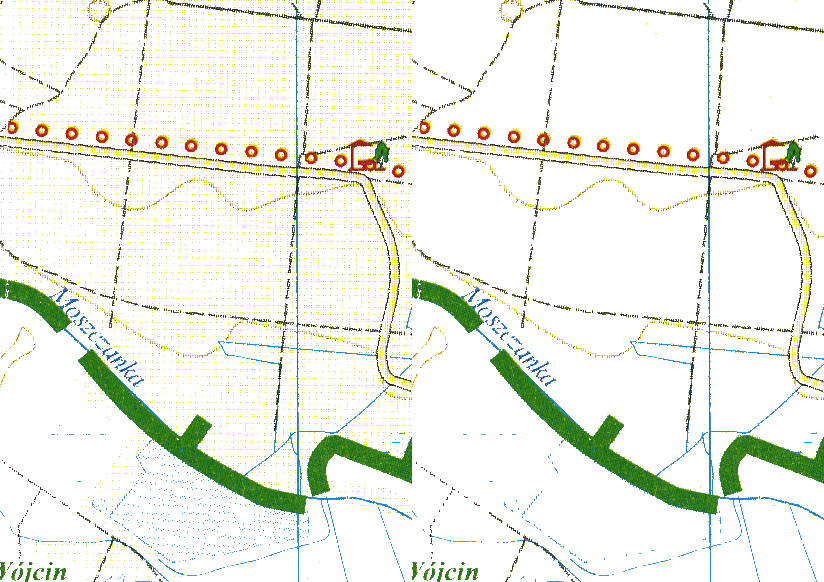
\includegraphics[scale=0.4]{images/removeLonePixelsResult.png}
\caption{Fragment of a map of Brzeg with lonely pixels removal algorithm applied.
On the left, there is a thresholded image. On the right side there is an image with removed
lonely pixels.}
\label{removeLonePixelsResult}
\end{center}
\end{figure}

In the second part of the quality improval method, the unsharp mask is applied to remove input
distortions, mainly to merge broken lines and improve text readability. Unsharp mask is applied with
a very small value of its parameters. Example output of this algorithm is presented in a 
Fig.~\ref{unsharpMaskResult}. All details, especially thin lines are clearer.

\begin{figure}[!ht]
\begin{center}
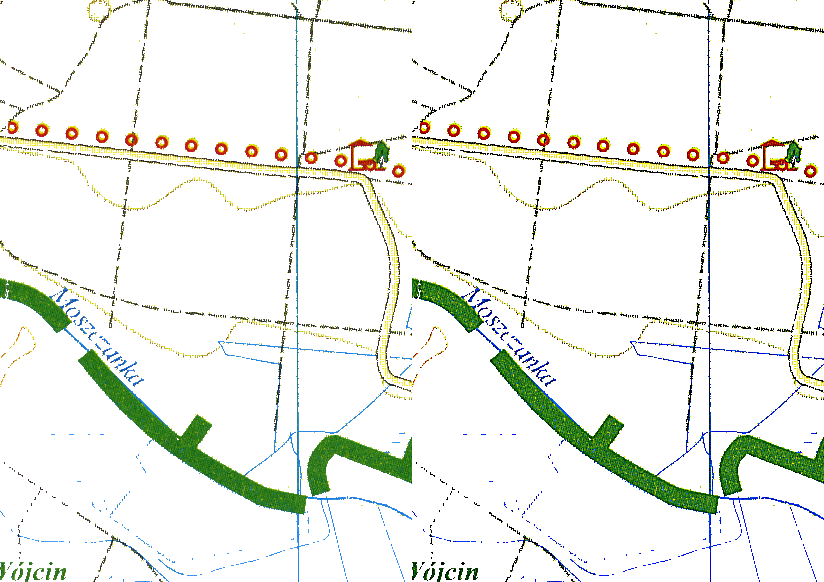
\includegraphics[scale=0.4]{images/unsharpMaskResult.png}
\caption{Fragment of a map of Brzeg with unsharp mask algorithm applied.
On the left, there is an image with previous algorithms applied. On the right side there is an image
with Unsharp Mask applied.}
\label{unsharpMaskResult}
\end{center}
\end{figure}

\subsubsection{Elements classification}

Elements classification algorithm is divided to four parts. First, image is initialy filtered. Then
all image elements are detected and assigned in a resulting image. Finally, to improve an output
quality, White Noise elimination algorithm is applied.

During the filtration process of an input map, there are applied two filters - Gaussian and
Bilateral. The first one is called with a very small value of radius and standard deviation. The
second one is applied with small values of diameter and sigma space. Sigma color value is bigger,
its value depends on the type of the map. Initial filtration of the map is done to unify colors of
each element type. Thanks to this method segmentation process is easier. Example of previously
thresholded map filtration is shown in a Fig.~\ref{contoursFiltrationResult}. As it can be seen,
color of every element is unfied. Thanks to usage of small parameter values, text is still readable.

\begin{figure}[!ht]
\begin{center}
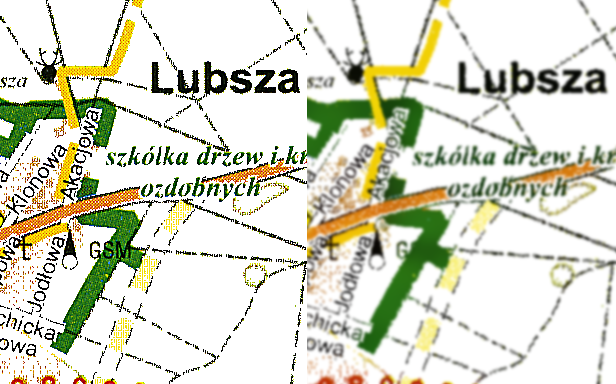
\includegraphics[scale=0.6]{images/filtrationResult.png}
\caption{Fragment of a map of Brzeg with filtration algorithms applied.
On the left, there is an image with previous algorithms applied. On the right side there is a
filtered image.}
\label{contoursFiltrationResult}
\end{center}
\end{figure}

In the second part of the algorithm all elements are detected. It is done in similar way as in
background detection (presented in Algorithms~\ref{colorGroupingAlgorithm},~\ref{groupsMergingAlgorithm}
~and~\ref{colorAssignmentAlgorithm}). It is assumed, that the same elements are equally colored in
the input. There are created groups of colors on the basis of previously processed image. White
elements  (removed background in thresholded image is marked in this color) are omitted. After this
process, every non-white element of thresholded image is assigned to one of created groups.

In the last part of the procedure, there is applied Fast Nl Means Denoising algorithm to remove
white noise from the result. It improves quality of the method output. Denoising factor parameter
used in this part is small.

Example of elements detection algorithm is presented in a Fig.~\ref{lineDetectionResult}. As it can
be seen, all background has been removed. Detected elements are consistent, all details are clear
and undamaged. Color of every element is unified. Text is clear and readable. Roads and rivers
 (thin lines) are visible and not broken.

\begin{figure}[!ht]
\begin{center}
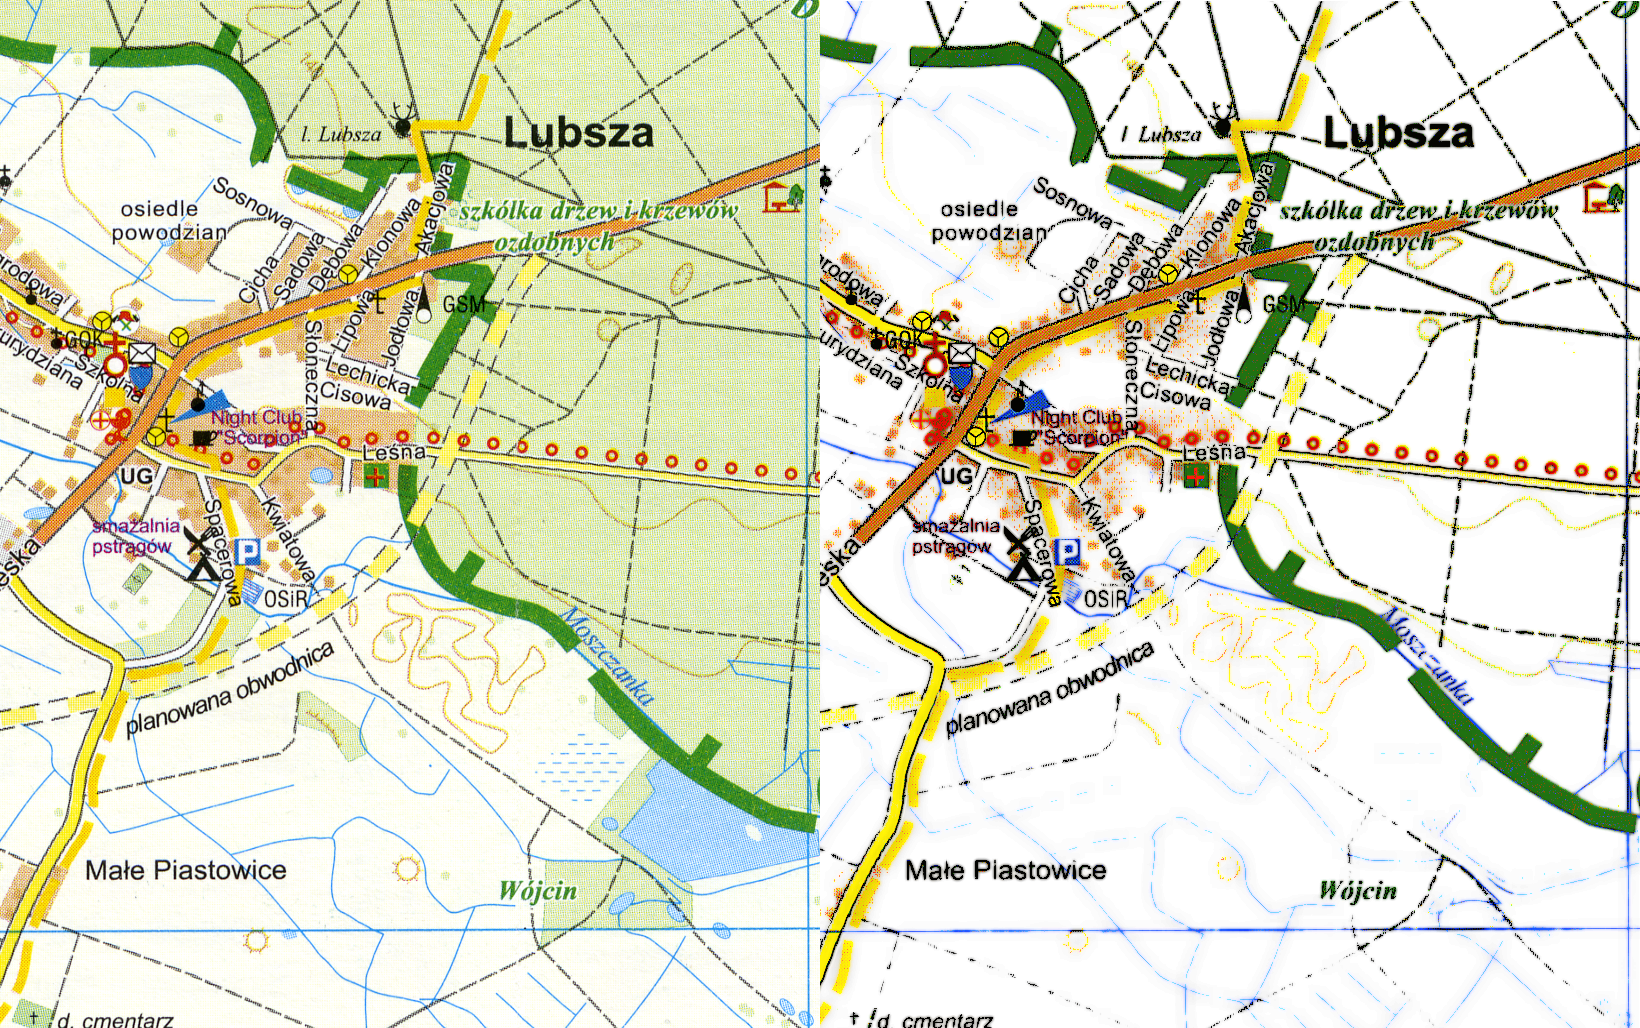
\includegraphics[scale=1.2]{images/lineDetectionResult.png}
\caption{Fragment of a map of Brzeg with Elements Detection (all parts) applied.
On the left, there is an image input map. On the right side there is a resulting image.}
\label{lineDetectionResult}
\end{center}
\end{figure}

\subsection{Algorithm parameters}
\label{lineDetectionParamsSection}

Similarly like in background detection algorithm, detection of details requires the specification of
some parameters. Their value depend on the type of the map.

\begin{description}
  \item[enabled] \hfill \\
    Determines, if Background Detection algorithm is enabled. \\
    Possible~values:~\{\textit{true},~\textit{false}\};
  \item[threshold\_value] \hfill \\
    Value of the threshold used by Thresholding algorithm. \\
    Possible~values:~integer~number. Proposed~values:~[80~-~150];
  \item[unsharp\_mask\_standard\_deviation] \hfill \\
    Standard deviation used by the Unsharp Mask algorithm. \\
    Possible~values:~integer~number. Proposed~values:~[0~-~5];
  \item[denoising\_factor] \hfill \\
    Denoising Factor parameter used in white noise elimination. \\
    Possible~values:~integer~number. Proposed~values:~[30~-~50];
  \item[bilateral\_filter\_counter] \hfill \\
    Number of bilateral filter applications. \\
    Possible~values:~integer~number. Proposed~values:~[0~-~3];
  \item[gaussian\_blur\_radius] \hfill \\
    Radius of a Gaussian Blur. \\
    Possible~values:~integer~number. Proposed~values:~[5~-~15];
  \item[gaussian\_blur\_standard\_deviation] \hfill \\
    Standard deviation of a Gaussian Blur. \\
    Possible~values:~integer~number. Proposed~values:~[0~-~5];
  \item[gaussian\_blur\_counter] \hfill \\
    Number of applications of Gaussian Blur algorithm. \\
    Possible~values:~integer~number. Proposed~values:~[0~-~3];
  \item[initial\_threshold] \hfill \\
    Initial threshold used by elements detection algorithm \\
    Possible~values:~integer~number. Proposed~values:~[5~-~15];
  \item[mimimal\_color\_area] \hfill \\
    Minimal number of elements classified as one group. \\
    Possible~values:~integer~number. Proposed~values:~[500~-~1000];
  \item[max\_number\_of\_colors] \hfill \\
    Maximum number of detected unique elements. \\
    Possible~values:~integer~number. Proposed~values:~[5~-~15];
  \item[diameter] \hfill \\
    Diameter used by Bilateral Filter. \\
    Possible~values:~integer~number. Proposed~values:~[20~-~40];
  \item[sigma\_color] \hfill \\
    Sigma Color used by Bilateral Filter. \\
    Possible~values:~integer~number. Proposed~values:~[100~-~150];
  \item[sigma\_space] \hfill \\
    Sigma Space used by Bilateral Filter. \\
    Possible~values:~integer~number. Proposed~values:~[30~-~70];
\end{description}

\section{Merge of layers}

Outputs of the area detection and the details detection algorithms are separate images. When these
two parts finish its work, produced results should be merged into one image. This procedure is very
simple and it is based on assumption, that the background of details detection algorithm is white.
If color of pixel from the detail detection result image is white, pixel from background detection
algorithm result is taken. Pseudocode of Merge Layer procedure is presented in the 
Algorithm~\ref{mergeLayersAlgorithm}.

\begin{algorithm}[!ht]
  \KwIn{AreaDetectionOutput}
  \KwIn{DetailsDetectionOutput}
  \KwOut{MergedImage}

  MergedImage := DetailsDetectionOutput\;

  \ForEach{PixelPosition in MergedImage}
  {
    \If{ DetailsDetectionOutput.at(PixelPosition).isWhite() }
    {
      MergedImage.at(PixelPosition).color := AreaDetectionOutput.at(PixelPosition).color\;
    }
  }

  \Return{MergedImage}

  \caption{Layers merge}
  \label{mergeLayersAlgorithm}
\end{algorithm}

In a Fig.~\ref{layerMergeResult}, there is an example result of a Layer Merge. As it can be seen,
all white areas from Details Detection result image (left) were substituted with colors from
corresponding areas from Background Detection result image (central). The result of merging can be
seen on the right image.

\begin{figure}[!ht]
\begin{center}
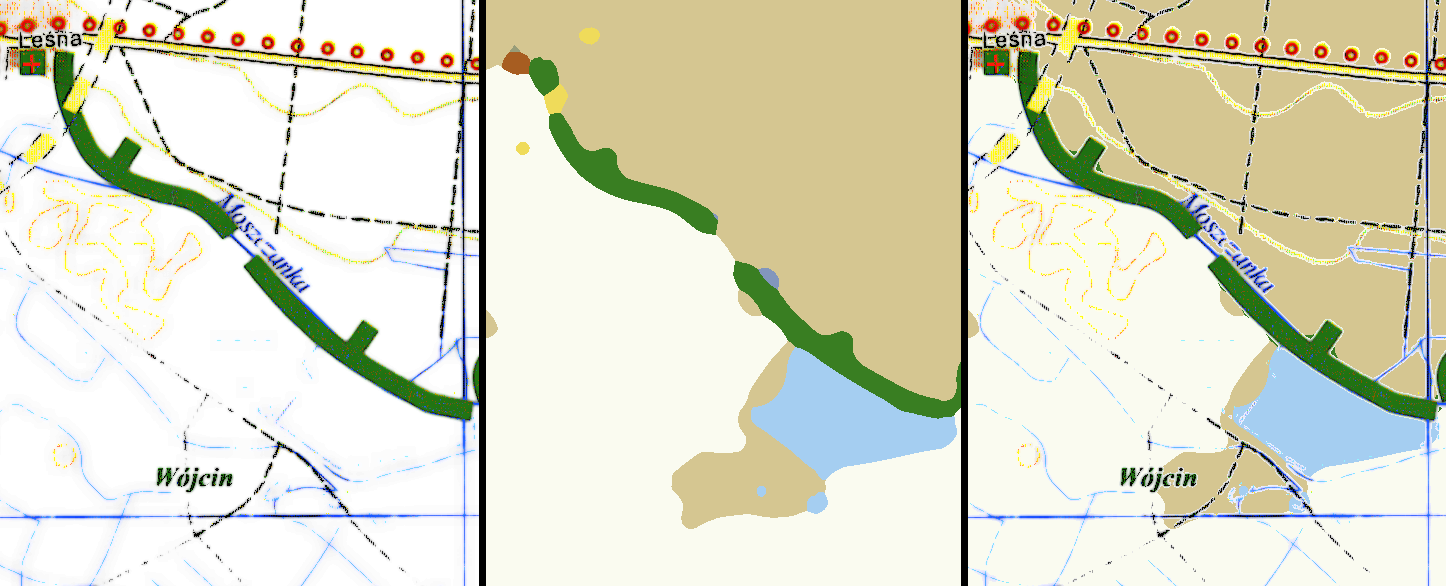
\includegraphics[scale=0.3]{images/layersAndMergedImage.png}
\caption{Fragment of a map of Brzeg with Layer Merge algorithm applied.
DetailsDetection result is represented on Left Image. Central image is
BackgroundDetection result. On the right, there is Layer Merge result.}
\label{layerMergeResult}
\end{center}
\end{figure}

\chapter{Implementation of the algorithm}

This chapter focuses on the engineering part of the work. First, there is a description of all used
tools in an implementation process. In the second part, the description of all classes and
their implementation is given.

\section{Used tools}

This section provides descriptions and versions of programming language, tools and libraries, which
were used during development process.

\subsection{Programming Language and Building Process Management}

All implementation of the master thesis application is developed in \textit{C++} programming 
language. It was choosen because of its high performance and availability of many useful libraries.
Used compiler is GCC in version 4.6.3. \\

For the managing the building process, \textit{CMake} was used. It fits very well to the
characteristics of the project - it supports directory hierarchies and library dependencies.
Moreover, this software is compiler-independent, so project can be compiled on multiple platforms,
like Linux, Microsoft Windows or Apple iOS. CMake documentation and download page is available on
\cite{cmakeMainPage}.

\subsection{External libraries}
\label{externalLibrariesSection}
To facilitate the development process there are used four external libraries in the project:
\textit{OpenCV} for digital image processing, \textit{RapidXML} for managing XML files,
\textit{Boost} and \textit{STL} for general purpose tools.

\subsubsection{OpenCV}

According to \cite{learningOpenCv}, OpenCV is an open-source computer vision library. It is written
in C and C++ and runs on multiple platforms. It was designed for computational efficiency with a
strong focus on real-time applications. It provides a simple to use computer vision architecture
and Machine Learning Library. It contains over 500 functions, that span many areas in vision. It is
used in many commercial and open-source projects. OpenCV documentation and download page can be
found on \cite{opencvMainPage}. This project uses OpenCV in version 2.4.9.

\subsubsection{Boost}

According to \cite{boostWiki}, Boost is a set of libraries for the C++ programming language. It 
contains over eighty individual libraries, which provide support for many tasks and structures.
In this work, there were used five libraries from Boost:
\begin{itemize}
  \item Boost Smart Pointers - objects, which store pointers to dynamically allocated (heap) objects;
  \item Boost Filesystem - library provides facilities to manipulate files and directories, and the
        paths that identify them;
  \item Boost Thread - library enables the use of multiple threads of execution with shared data in
        portable C++ code;
  \item Boost Foreach - Foreach loop designed for C++;
  \item Boost Posix Time - Library defines a non-adjusted time system with nano-second/micro-second
        resolution and stable calculation properties.
\end{itemize}

Boost documentation and download page can be found on \cite{boostMainPage}. This project uses Boost
in version 1.46.

\subsubsection{STL}

According to \cite{stlWiki}, Standard Template Library (STL) is a software library for the C++
programming language. It provides four components called algorithms, containers, functional and
iterators. It is a part of a C++ standard.

\subsubsection{RapidXML}

RapidXML is a fast XML DOM parser for C++ Programming Language. Its documentation and download page
can be found on \cite{rapidXmlMainPage}. This project uses RapidXML in version 1.13.

\section{Application outline}

This section provides descriptions of application design and main classes and interfaces implemented
during the development process.

\subsection{Application design}

The application code is divided into 6 packages:

\begin{enumerate}
  \item Algorithm - This package contains class, which controls main flow of a filtration and
        segmentation algorithm;
  \item Core - This package contains the \textit{main.cpp} file. Application work starts here;
  \item Debug - Package contains a class, which views input and output images on a screen of the
        computer. To enable this package, \textit{-DDEBUG\_IMAGES} definition should be added to
        compilation process of the application.
  \item Filehandler - Classes included in this package are responsible for an Input/Output
        operations: finding path to the input images, loading an input image, finding path to the
        output images, loading an output image and loading an XML configuration file;
  \item Filtration - This package contains classes responsible for an image filtration. Every
        filtration algorithm is represented by a separate class;
  \item Segmentation - This package contains classes responsible for an image segmentation. Every
        segmentation algorithm is represented by a separate class. It contains also one subpackage,
        called \textit{helpers}, which includes classes helping in a segmentation process.
\end{enumerate}

All application architecture is visualized in a Fig.\ref{classDiagramImage}.

\begin{figure}[!ht]
\begin{center}
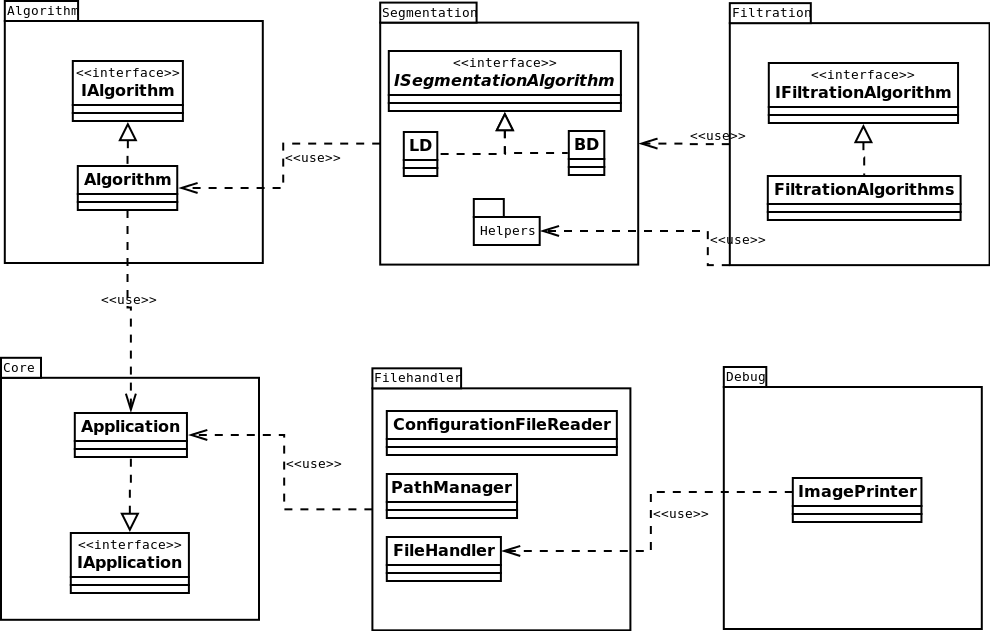
\includegraphics[scale=0.4]{images/classDiagram.png}
\caption{Application architecture.}
\label{classDiagramImage}
\end{center}
\end{figure}

\subsection{Description of main classes and interfaces}

This section focuses on description of most important classes included in core, algorithm,
filtration and segmentation packages.

\subsubsection{core::Application}

This class starts at the beggining and is running for all the time. It controls main flow of the
application. First, it reads all parameters from the configuration XML file (using 
\textit{filehandler::ConfigurationFileReader} class). Next, it loads every input image. Finally, for
each loaded map it starts an algorithm and saves its result to an output file. Reading input and
saving output of the algorithm is done using \textit{filehandler::FileHandler} class. The map
segmentation and filtration algorithm process is controlled by \textit{algorithm::Algorithm} class.

\subsubsection{algorithm::Algorithm}

This class controls the flow of the Detail Detection, Background Detection and Layer Merge
algorithms. First, algorithm checks, which algorithms are enabled. Next, proper algorithms are run.
Finally, class prepares an output image (it decides, if layer merging is needed).

\subsubsection{segmentation::ISegmentationAlgorithm}

It is the interface for all classes controling a segmentation process. It has two implementations:
\begin{itemize}
  \item \textit{segmentation::LineDetection} - This class is responsible for the Detail Detection
        process;
  \item \textit{segmentation::ColorSegmentation} - This class is responsible for the Background
        Detection process.
\end{itemize}

Classes, which implement this interface should have overrided one method:

\begin{lstlisting}[language=C++, caption=ISegmentationAlgorithm methods]
virtual boost::shared_ptr<cv::Mat> apply( boost::shared_ptr<cv::Mat> ) const = 0;
\end{lstlisting}

It takes a \textit{shared\_ptr} to an input image and returns
\textit{shared\_ptr} to an output, segmented image.

\subsubsection{filtration::IFiltrationAlgorithm}

This interface unifies usage of every filtration algorithm. It is implemented by nine classes:
\begin{itemize}
  \item \textit{ApplyBilateralFilter} - This class applies Bilateral Filter to an image;
  \item \textit{ApplyGaussianFilter} - This class applies Gaussian Filter to an image;
  \item \textit{ConvertToBlackAndWhite} - This class converts an image to black and white mode;
  \item \textit{Dilation} - This class applies Dlation to an image;
  \item \textit{ElliminateWhiteNoise} - This class eliminates white noise from an image;
  \item \textit{Erosion} - This class applies Erosion to an image;
  \item \textit{RemoveLonePixels} - This class applies filter, which removes lonely pixels from an
        image;
  \item \textit{Threshold} - This class applies Thresholding to an image;
  \item \textit{UnsharpMask} - This class applies an Unsharp Mask filter to an image.
\end{itemize}

Classes, which implement this interface, should have overriden one method:

\begin{lstlisting}[language=C++, caption=IFiltrationAlgorithm methods]
virtual boost::shared_ptr<cv::Mat> apply( boost::shared_ptr<cv::Mat> ) const = 0;
\end{lstlisting}

It takes a \textit{shared\_ptr} to an input image and returns
\textit{shared\_ptr} to an output, segmented image.

\section{Running the application}

This section focuses on compilation and application running processes for a Linux OS.

\subsection{Compilation and running}

To compile the application properly, there are needed CMake, Boost and OpenCV in proper versions (
listed in section~\ref{externalLibrariesSection}). CMake checks the dependencies in the system and
generates a Makefile. If this process is successful, it is possible to start the compilation.

\begin{lstlisting}[language=sh, caption=Commands needed for building the application]
# Application root Directory
$ cmake . # It runs the CMake, checks dependencies and generates the Makefile
$ make # This command compiles application.
\end{lstlisting}

After successful compilation, the binary file should appear in a \textit{(project\_root)/bin/}
directory. To run it, the binary file should be executed:

\begin{lstlisting}[language=sh, caption=Commands needed for running the application]
# Application root Directory
$ ./bin/MasterThesisWojciechowski
\end{lstlisting}

\subsubsection{Scripts}

To ease process of compilation and running, three scripts are prepared:

\begin{itemize}
  \item \textit{clean.sh} - script removes all application output files, application binaries and
        CMake files;
  \item \textit{fast\_compile\_and\_run.sh} - Script compiles the project and starts the application;
  \item \textit{compile\_and\_run.sh} - Scripts does everything from \textit{clean.sh} and
        \textit{fast\_compile\_and\_run.sh};
\end{itemize}

\subsection{Input and output files}

All input and output files are placed in a \textit{(project\_root/resources/)} directory.

\subsubsection{Configuration file}

All parameters of the algorithm should be given in a configuration file, which full path must be:~
\textit{(project\_root)/resources/conf/config.xml}. This file is divided into two parts (xml nodes)
to improve its readability. First node:~\textit{background\_detection} contains all arguments for
Background Detection algorithm. Second node:~\textit{line\_detection} contains all arguments for
Details detection algorithm. Description of all parameters can be found in
sections:~\ref{backgroundDetectionParamsSection}~and~\ref{lineDetectionParamsSection}.

On al listing below there is an example of a \textit{config.xml} file:

\begin{lstlisting}[language=xml]
<?xml version="1.0" encoding="UTF-8"?>
<configuration>
    <background_detection>
        <enabled>true</enabled>
        <gaussian_blur_radius>13</gaussian_blur_radius>
        <gaussian_blur_standard_deviation>0</gaussian_blur_standard_deviation>
        <diameter>10</diameter>
        <sigma_color>150</sigma_color>
        <sigma_space>150</sigma_space>
        <dilation_and_erosion_size>1</dilation_and_erosion_size>
        <dilation_and_erosion_counter>5</dilation_and_erosion_counter>
        <window_width>20</window_width>
        <max_number_of_colors>30</max_number_of_colors>
    </background_detection>

    <line_detection>
        <enabled>true</enabled>
        <threshold_value>110</threshold_value>
        <unsharp_mask_standard_deviation>5</unsharp_mask_standard_deviation>
        <denoising_factor>35</denoising_factor>
        <bilateral_filter_counter>5</bilateral_filter_counter>
        <gaussian_blur_radius>9</gaussian_blur_radius>
        <gaussian_blur_standard_deviation>3</gaussian_blur_standard_deviation>
        <gaussian_blur_counter>5</gaussian_blur_counter>
        <initial_threshold>10</initial_threshold>
        <mimimal_color_area>500</mimimal_color_area>
        <max_number_of_colors>15</max_number_of_colors>
        <diameter>25</diameter>
        <sigma_color>130</sigma_color>
        <sigma_space>50</sigma_space>
    </line_detection>
</configuration>
\end{lstlisting}

\subsubsection{Input and output images}

Every input map (it can be more than one) should be placed in a \textit{resources/input\_images}
directory. Images must be placed there before starting the application. There are acceptable all
file formats, which are supported by OpenCV library (for example \textit{jpg}, \textit{tif},
\textit{bmp}).
When application finishes its work, the result is saved in a \textit{resources/output\_images}
directory. Saved images have the same name and format as their input equivalents.

\chapter{Tests and Results}

This chapter contains description of all tests of created algorithm. In the second part there are
presented results of made tests and their analysis.

\section{Test description}

\subsection{Scope of tests}

Tests were made for each picture with different values of parameters. There are two properties
tested. First is a quality of an output image. During this phase there are checked such properties
like: proper borders of each area, proper color of the area, presence of all small details,
continuities of lines (in roads, rivers, etc.) and readability of text. Second checked property is
the algorithm performance. There was checked time of execution of the algorithm. Measurement is
divided into three categories:
\begin{enumerate}
  \item Time of Details Detection algorithm;
  \item Time of Background Detection algorithm;
  \item Time of execution of both algorithms.
\end{enumerate}

Images were divided into groups according to the best achieved image quality. All pictures from one
group were tested with the same set of algorithm parameters.

\subsection{Test environment}

Description of the computer on which all tests were done is presented in the
Table~\ref{computerDescription}.

\begin{table}[!ht]
\begin{center}
\caption{Test environment.}
\label{computerDescription}
\begin{tabular}{|c|c|}
  \hline
  CPU & Intel Core 2 Duo T6600 @ 2.20GHz x 2 \\
  \hline
  Memory & 4GB RAM \\
  \hline
  Operating System & Ubuntu Linux 12.04 (precise) 64-bit \\
  Kernel & 3.8.0-42-generic \\
  Desktop Environment & Gnome 3.4.2 \\
  \hline
\end{tabular}
\end{center}
\end{table}

\subsection{Input data}

To confirm proper working of the algorithm, there were nine maps prepared. All input map files
with their description are listed in a table~\ref{tableInputFiles}. 

\begin{table}[!ht]
\begin{center}
\caption{Input files.}
\label{tableInputFiles}
\begin{tabular}{|c|c|c|c|}
  \hline
  Filename & Format & Resolution & Description \\
  \hline
  brzeg & tif & 3391x4671 & Geographical map of Brzeg. It has text and multiple \\
        &     &           & areas like forests, lakes, roads and cities \\
  \hline
  bydgoszcz & bmp & 1747x1272 & City map of Bydgoszcz. Small number of areas, \\
            &     &           & high density of roads and small details \\
  \hline
  dolny\_slask & png & 5936x8669 & Old map of a Lower Silesia. No backround. \\
              &     &           & Many thin lines and rivers. \\
  \hline
  lubsza & tif & 3391x4671 & Geographical map of surroundings of Lubsza. \\
         &     &           & It has many areas like forests and lakes. Image has \\
         &     &           & a big damage. Map was bent during scanning process. \\
  \hline
  masyw\_slezy & tif & 3883x4606 & Topographic map of Ślęża Mountain. It contains \\
              &     &           & many areas in different colors, roads, text and \\
              &     &           & topographic lines. \\
  \hline
  namyslow & jpg & 4814x5628 & Topographic map of Namysłów. It contains many \\
           &     &           & small details, topographic lines, small text  \\
           &     &           & and bright background of areas\\
  \hline
  pokoj & tif & 2921x2989 & Geographical map of Pokój. It has text, \\
        &     &           & multiple areas (forests, lakes) and roads. \\
  \hline
  sleza & jpg & 1812x2756 & Geographical map of Ślęża. It contains \\
        &     &           & areas like forests, lakes and roads. \\
  \hline
  sobotka & png & 2798x1824 & Geographical map of Sobótka. It has many \\
          &     &           & different areas, like small details, text and roads. \\
  \hline
\end{tabular}
\end{center}
\end{table}

\section{Result analysis}

Testing process was divided into six groups. Every group had different parameters set during testing
process. Results, which are presented in this section are the best achieved for each map (among
all tests with different values of parameters).

\subsection{Ślęża and Sobótka}

Ślęża and Sobótka are geographic maps designed for tourists. They are taken from atlas. Map of 
Sobótka has streets with their names, travel routes and some small details. It contains areas of a
park, small lakes and smaller areas in the city. On Ślęża map there are marked mainly travel routes,
names of places, which are worth seeing and area of the park and a city.

\subsubsection{Used parameters}

Background of these maps have visible moro effect and some distortions (dust). To eliminate them,
there was used a Gaussian Blur with a big radius - 15. Diameter of a bilateral filter was set to
20, its sigma space to 75 and sigma color to 150. To keep the shape of areas, remove all details
and not needed lines, dilation and erosion was applied once, with small size - 1. Holes removal
algorithm was used with a window width set to 10 - there were many residues in an image after
application of erosion and dilation. Maximum numbers of colors parameter was set to 30. It is enough
value for the background. \\

Details detection was set to medium-sensitive. Threshold was set to 110. It was enough to keep all
details and lines with this value, background and distortions have been successfully eliminated.
To improve image quality, standard deviation of unsharp mask was set to 5 and denoising factor to
35. Image filtering was quite big as for details detection. It was caused by the moro effect inside
the green area, which was hard to eliminate. Bilateral filter was applied five times with diameter =
20, sigma color = 150 and sigma space = 50. Gaussian filter was applied two times with a radius = 7.
Image contains small number of colors. Maximal number of colors parameter was set to 12 and initial
threshold to 10. Minimal color area was set to 500, because images has big resolution.

\subsubsection{Achieved results}

The result of application of the algorithm on Ślęża map is presented in a Fig.~\ref{resultSlezaIO}.

\begin{figure}[!ht]
\begin{center}
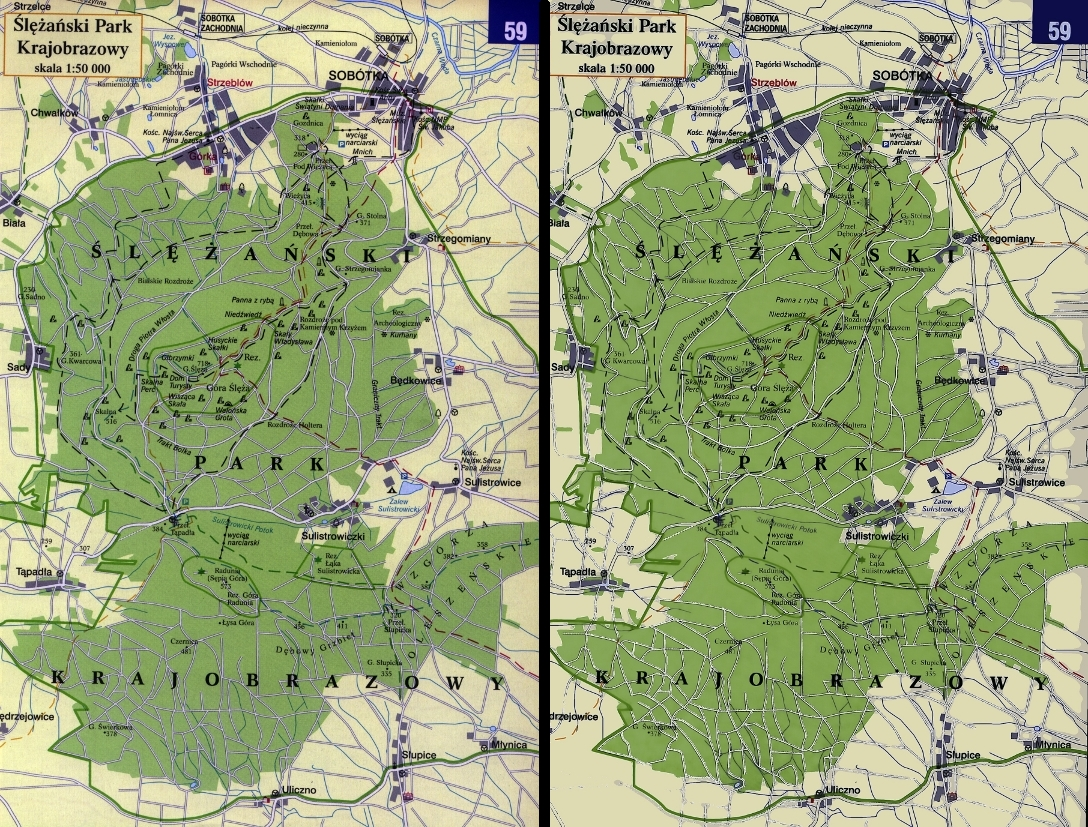
\includegraphics[scale=1.5]{images/resultSlezaIO.jpeg}
\caption{Result of application of the algorithm to Ślęża map. Original map is on the left, algorithm
result is presented on the right.}
\label{resultSlezaIO}
\end{center}
\end{figure}

Borders of the areas remained unchanged. Color is unified, distortions have been eliminated from
resulting image. All small details are kept and marked in a result image. There are also some 
errors. Near roads and bigger text, areas were assigned to wrong groups. It is especially visible on
the right center border of the map (it is marked in darker color). The same situation is visible
near text "Ślężański Park Krajobrazowy". It is caused by dilation and erosion algorithms application
 (surroundings of these areas are darker in the original - black text and roads). This situation is
presented in a Fig.~\ref{badBackgroundSleza}. 

\begin{figure}[!ht]
\begin{center}
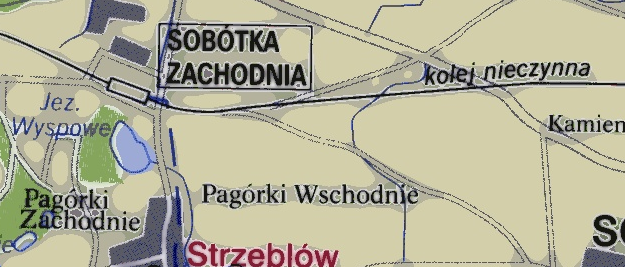
\includegraphics[scale=0.5]{images/badBackgroundSleza.png}
\caption{Wrong background color in enlarged Ślęża result.}
\label{badBackgroundSleza}
\end{center}
\end{figure}

Additionaly, on some areas (central green and grey near Górka town) it was
impossible to remove all moro effect. It is visible in a Fig.~\ref{moroSlezaIO}.

\begin{figure}[!ht]
\begin{center}
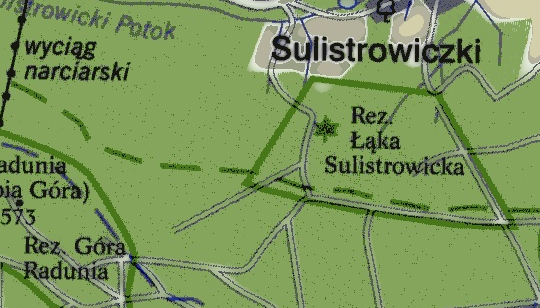
\includegraphics[scale=0.5]{images/moroSlezaResult.png}
\caption{Moro effect visible in enlarged Ślęża result.}
\label{moroSlezaIO}
\end{center}
\end{figure}

Area of the river is not continuous in all places. It is visible in a Fig.~\ref{slezaRiver}.

\begin{figure}[!ht]
\begin{center}
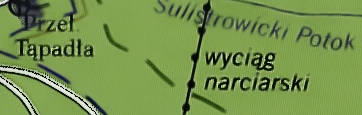
\includegraphics[scale=0.5]{images/slezaRozlanyTekst.png}
\caption{Not continuous river in Ślęża map.}
\label{slezaRiver}
\end{center}
\end{figure}

Performance of the algorithm is presented in a table \ref{slezaPerformance}.

\begin{table}[!ht]
\begin{center}
\caption{Time of algorithm execution - Ślęża.}
\label{slezaPerformance}
\begin{tabular}{|c|c|c|}
  \hline
  Detail Detection & Background Detection & Total Time \\
  \hline
  2 min 16s & 8 min 21s & 8min 21s \\
  \hline
\end{tabular}
\end{center}
\end{table}

The result of application of the algorithm on Sobótka map is presented in a
Fig.~\ref{resultSobotkaFinal}.

\begin{figure}[!ht]
\begin{center}
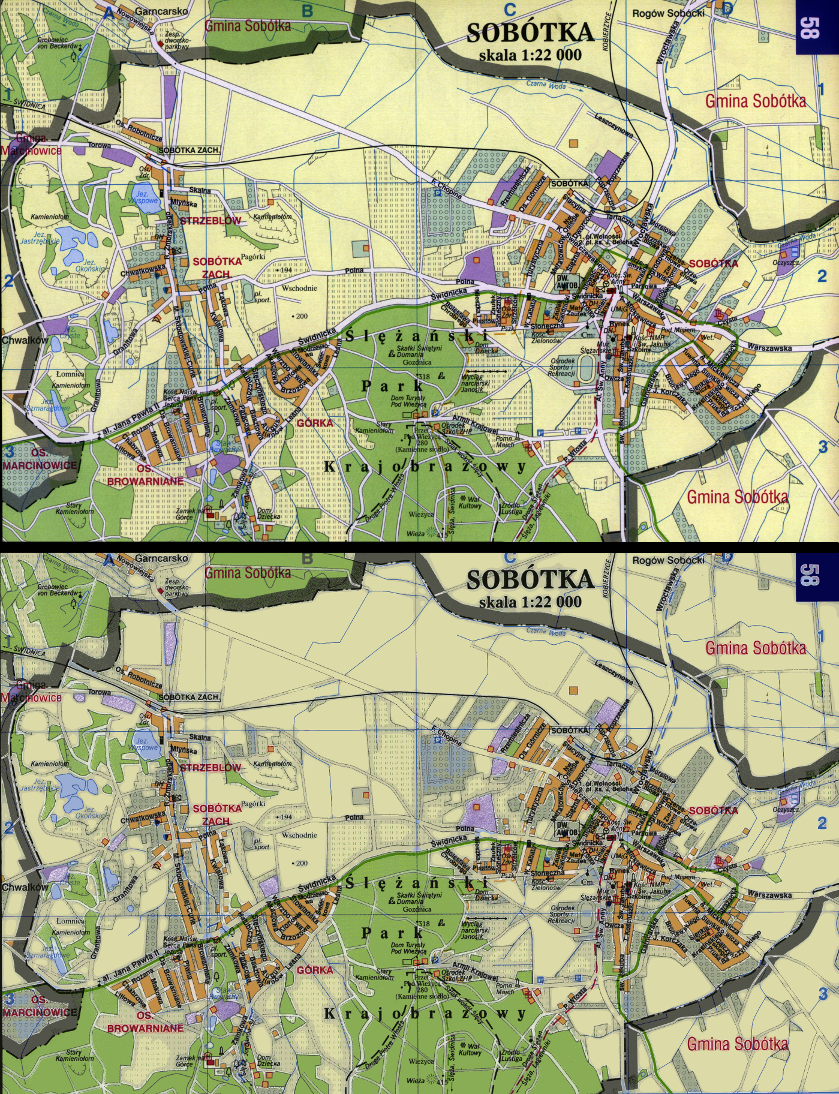
\includegraphics[scale=1.5]{images/resultSobotkaFinal.png}
\caption{Result of application of the algorithm to Sobótka map. Input map is on the upper part,
algorithm result is presented on the lower part.}
\label{resultSobotkaFinal}
\end{center}
\end{figure}

Borders of areas remained the same. All distortions have been eliminated (dust, second side of the
map). Text and small details are sharp and readable. Major part of the same areas have unified
color. Similarly to the Ślęża result, there are some areas with wrongly assigned color (presented in
a Fig.~\ref{sobotkaBadColorAssignment}) and there are some small remainings of a moro effect (
presented in a Fig.~\ref{sobotkaMoroEffect}). \\

\begin{figure}[!ht]
\begin{center}
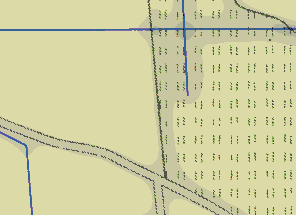
\includegraphics[scale=1.0]{images/sobotkaBadColorAssignment.png}
\caption{Badly assigned area in a Sobótka map.}
\label{sobotkaBadColorAssignment}
\end{center}
\end{figure}

\begin{figure}[!ht]
\begin{center}
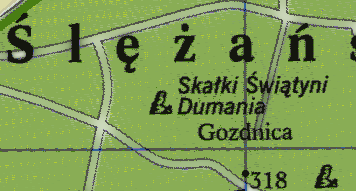
\includegraphics[scale=1.0]{images/sobotkaMoroEffect.png}
\caption{Moro effect in a Sobótka map.}
\label{sobotkaMoroEffect}
\end{center}
\end{figure}

Performance of the algorithm is presented in a table \ref{sobotkaPerformance}.

\begin{table}[!ht]
\begin{center}
\caption{Time of algorithm execution - Sobótka.}
\label{sobotkaPerformance}
\begin{tabular}{|c|c|c|}
  \hline
  Detail Detection & Background Detection & Total time \\
  \hline
  3 min 00s & 9 min 15s & 9min 15s \\
  \hline
\end{tabular}
\end{center}
\end{table}

Summarizing, the quality of segmentation of Ślęża and Sobótka maps is good. Despite some errors in
assigning a pixel to the color group, most of elements and areas are processed properly.

\subsection{Pokój}

Pokój is a map of a small town. There are marked streets with their names, bigger road and town
surroundings (multiple ponds and green areas). The map background is not consistent - there are 
visible big dots. It is an additional difficulty for an algorithm.

\subsubsection{Used parameters}

In case of this map the background does not have any distortions. The main difficulty is the moro
effect, which is present in a different form, than in other images. To eliminate this, there are
used filters with bigger values of parameters. Radius of a Gaussian blur is set to 9, diameter to
10, sigma color and sigma space to 50. Dilation and erosion is applied once with small size - 1.
Window width is also small and set only to 3. The map does not have many background colors. This
value is set to 15. \\

In the detail detection algorithm unusual moro effect is also a problem. With bigger threshold
values some dots are still visible. To ensure quality and sharpness of details or text and also to
remove dots from moro effect, the threshold value is set to 100. Unsharp mask standard deviation is
set to 5. Denoising factor is quite big - it is set to 35. Bilateral filter is called five times
with diameter set to 30, sigma color to 130 and sigma space to 50. Gaussian blur is called two times
with radius set to 5. Maximal number of colors is small - 8. Initial threshold is 10 and minimal
color area is 500.

\subsubsection{Achieved results}

The result of a segmentation is presented in a Fig.~\ref{pokojResult}.

\begin{figure}[!ht]
\begin{center}
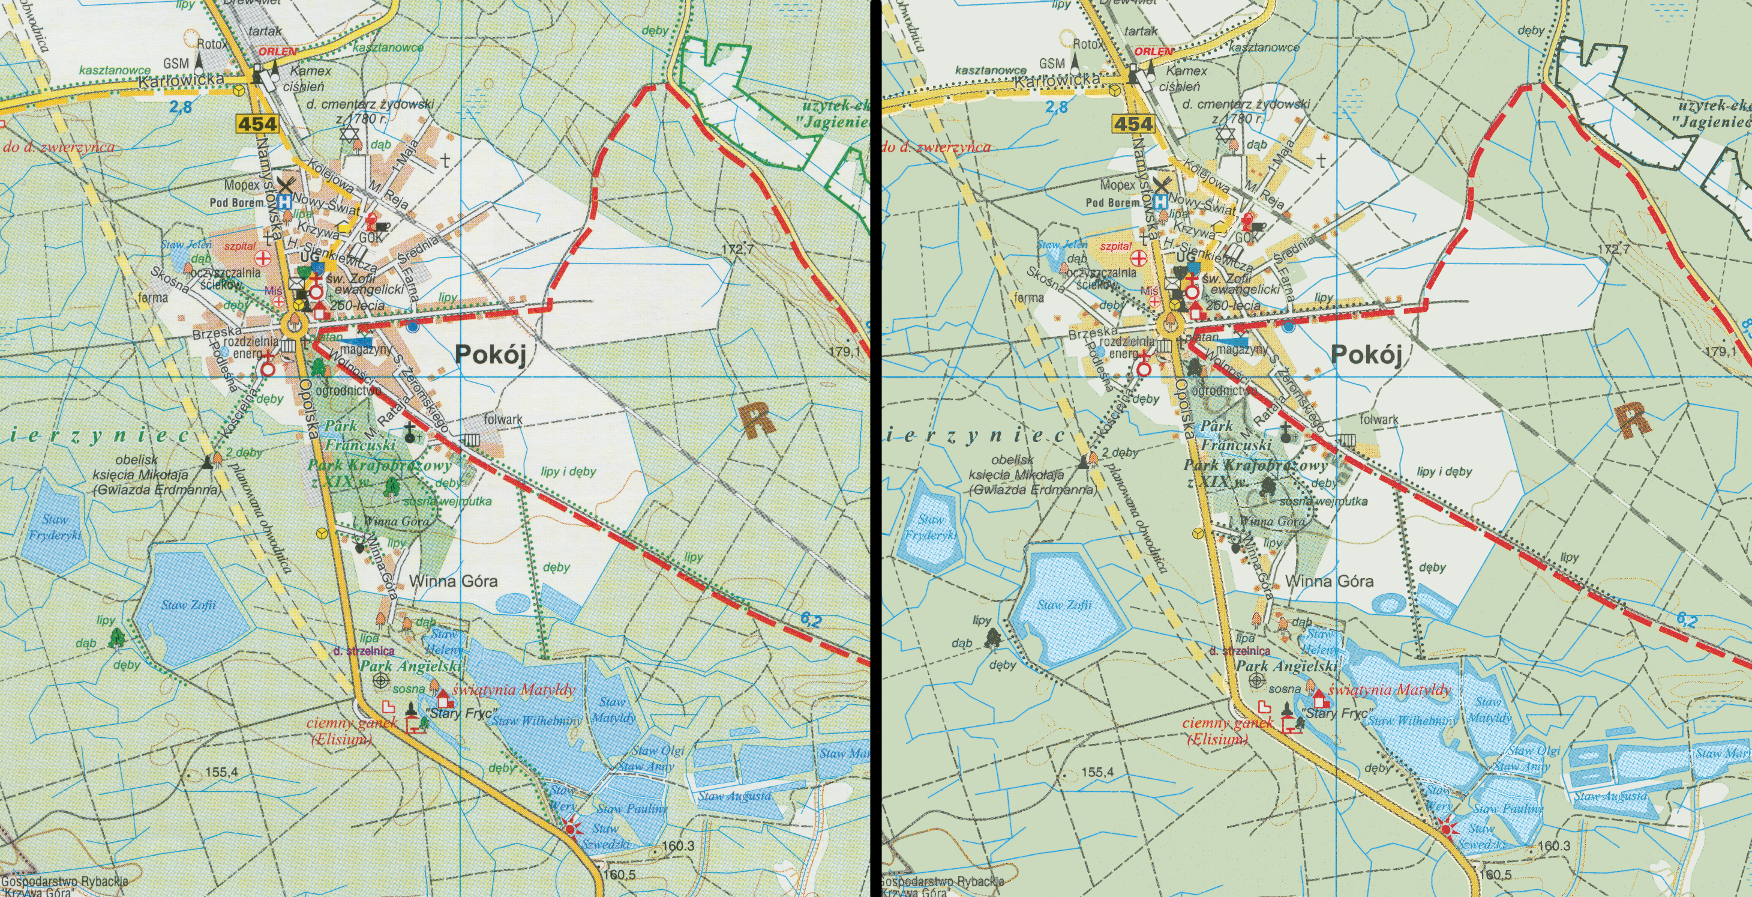
\includegraphics[scale=0.2]{images/pokojFinalResult.png}
\caption{Final result of the algorithm applied to Pokój map. Input image is on the left, the result
is on the right side of an image.}
\label{pokojResult}
\end{center}
\end{figure}

Size of the areas is correct. Almost all elements are segmented to proper groups. Text and small
details are visible, sharp and readable. Unfortunately moro effect in some places is too difficult
to segment out. It is especially visible near the lakes (shown in a Fig.\ref{pokojBadLake}) and in
the town (visualized in a Fig.~\ref{pokojBadCity}).

\begin{figure}[!ht]
\begin{center}
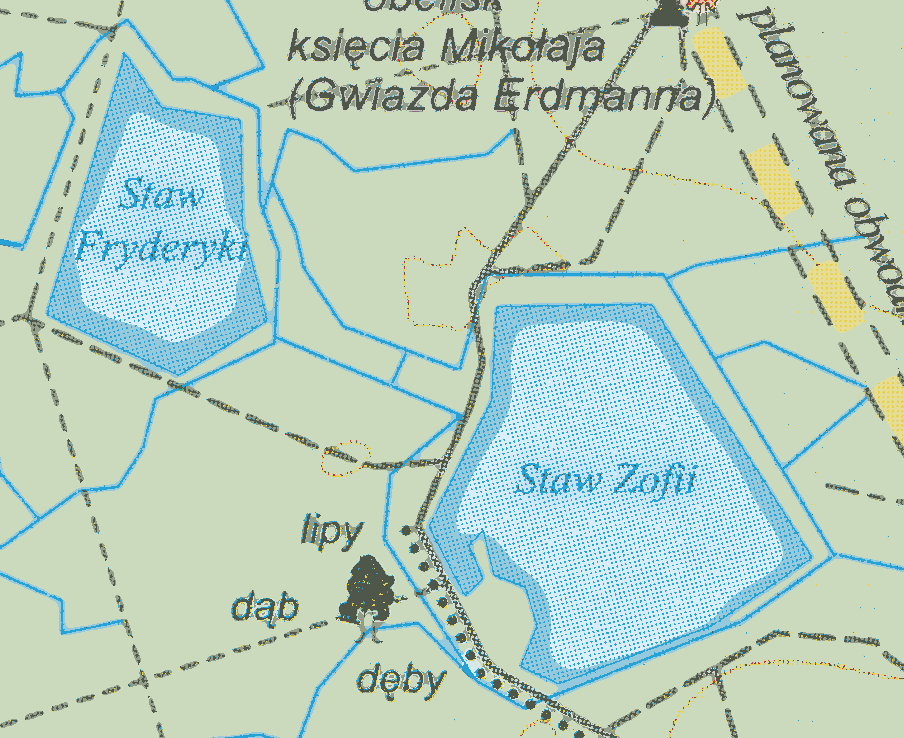
\includegraphics[scale=0.3]{images/pokojBadLake.png}
\caption{Moro effect visible in a Pokój map near the lake.}
\label{pokojBadLake}
\end{center}
\end{figure}

\begin{figure}[!ht]
\begin{center}
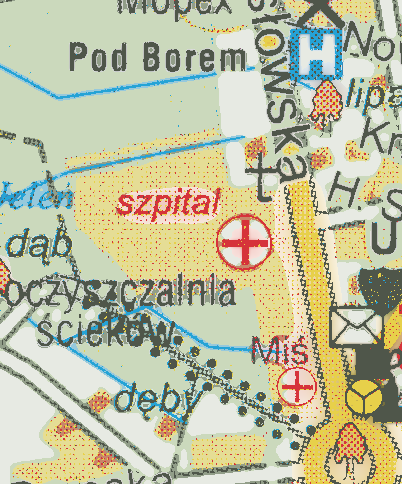
\includegraphics[scale=0.4]{images/pokojBadCity.png}
\caption{Moro effect visible in a Pokój map in the town.}
\label{pokojBadCity}
\end{center}
\end{figure}

Performance of the algorithm is presented in a table \ref{pokojPerformance}.

\begin{table}[!ht]
\begin{center}
\caption{Time of algorithm execution - Pokój.}
\label{pokojPerformance}
\begin{tabular}{|c|c|c|}
  \hline
  Detail Detection & Background Detection & Total Time \\
  \hline
  4 min 19s & 16 min 19s & 16min 19s \\
  \hline
\end{tabular}
\end{center}
\end{table}

\subsection{Lubsza and Brzeg}

Lubsza and Brzeg are geographical maps. There are visible green areas, towns with named streets,
rivers, roads, lakes and some thin lines. On some of the areas moro effect is visible (especially
after enlargement of images). There are many distortions visible on both maps. There are some
creases (one of them is major - in Lubsza map) and darker elements (result of improper scanning).

\subsubsection{Used parameters}

Maps of Lubsza and Brzeg have some distortions. To eliminate them there are used filters with a
bigger parameter values. Gaussian blur is applied with radius set to 13. Bilateral filter is
called with diameter set to 10, sigma color and sigma space set to 150. Dilation and erosion is
applied five times with a size set to 1. Holes are removed using a window width set to 30. Maps
have maximum 12 colors. \\

Lines are detected with a threshold set to 100. To improve quality of details, there is applied an
unsharp mask with standard deviation set to 5 and denoising factor set to 35. Gaussian blur is
applied twice with radius set to 5. Bilateral filter is applied five times with diameter set to 30,
sigma color to 130 and sigma space to 50. Map details are marked in maximum 10 colors. Initial
threshold is set to 10 and minimal color area is 500 (images have big resolution).

\subsubsection{Achieved results}

Result of the algorithm application in a map of Brzeg is presented in a Fig.~\ref{brzegResult}.

\begin{figure}[!ht]
\begin{center}
\includegraphics[scale=1.0]{images/brzegResultFinal.png}
\caption{Final result of the algorithm applied to Brzeg map. Input image is on the left, the result
is on the right side of an image.}
\label{brzegResult}
\end{center}
\end{figure}

Major part of areas and details is segmented properly. Text and details are sharp and readable.
Many distortions are eliminated. Unfortunately area inside the city of Brzeg is segmented wrongly.
It is shown in a Fig.\ref{badBrzeg}.

\begin{figure}[!ht]
\begin{center}
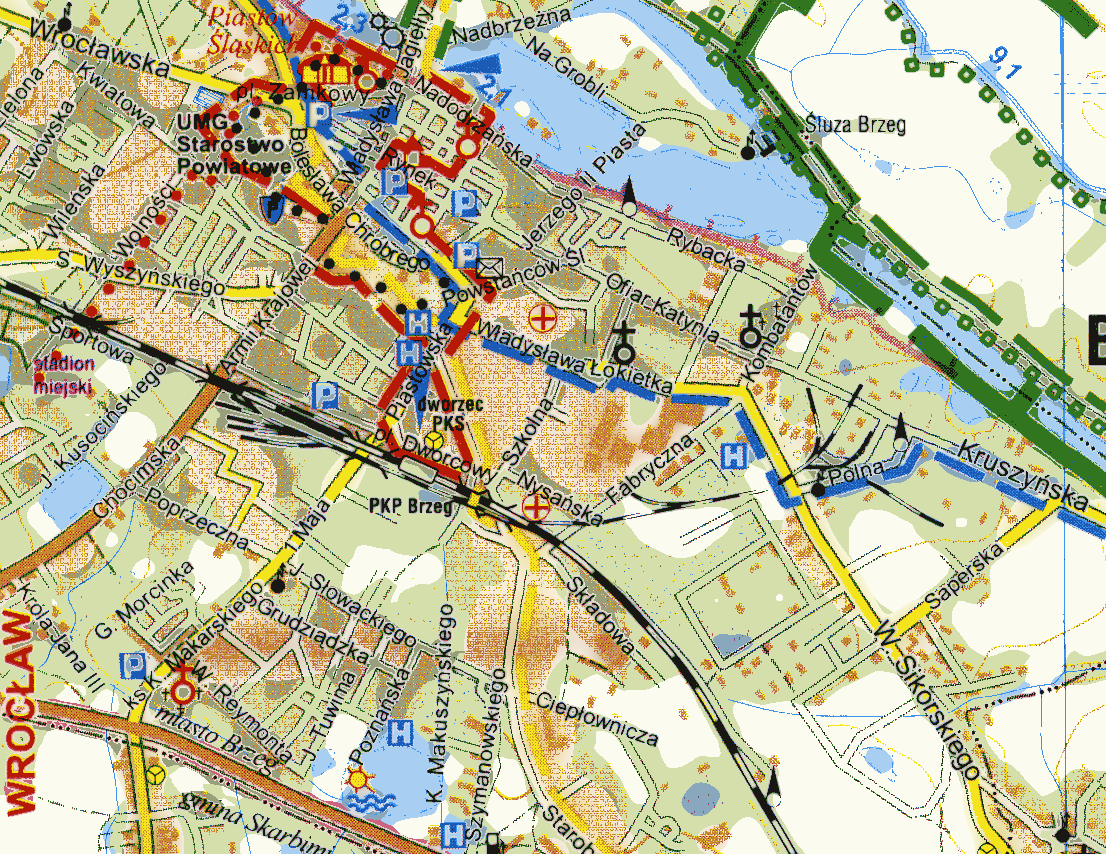
\includegraphics[scale=0.25]{images/badBrzeg.png}
\caption{Wrongly segmented areas inside Brzeg city.}
\label{badBrzeg}
\end{center}
\end{figure}

Additionaly, the river is not continuous in all places (situation visualized in a 
Fig.~\ref{badBrzegRiver}).

\begin{figure}[!ht]
\begin{center}
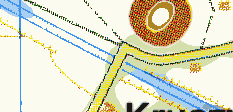
\includegraphics[scale=1.0]{images/badBrzegRiver.png}
\caption{Not continuous river in the map of Brzeg.}
\label{badBrzegRiver}
\end{center}
\end{figure}

Last, the moro effect inside main road is not eliminated (shown in a Fig.~\ref{badBrzegRoad}).

\begin{figure}[!ht]
\begin{center}
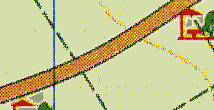
\includegraphics[scale=1.0]{images/badBrzegRoad.png}
\caption{Moro effect inside the road in the map of Brzeg.}
\label{badBrzegRoad}
\end{center}
\end{figure}

Performance of the algorithm is presented in a table \ref{brzegPerformance}.

\begin{table}[!ht]
\begin{center}
\caption{Time of algorithm execution - Brzeg.}
\label{brzegPerformance}
\begin{tabular}{|c|c|c|}
  \hline
  Detail Detection & Background Detection & Total Time \\
  \hline
  13 min 19s & 1h 7min 42s & 1h 7min 43s \\
  \hline
\end{tabular}
\end{center}
\end{table}

The result of application of algorithm on a Lubsza map is presented in a Fig.~\ref{lubszaResult}.

\begin{figure}[!ht]
\begin{center}
\includegraphics[scale=1.0]{images/lubszaResultFinal.png}
\caption{Final result of the algorithm applied to Lubsza map. Input image is on the left, the result
is on the right side of an image.}
\label{lubszaResult}
\end{center}
\end{figure}

Areas of this map are segmented very well. Also text and small details remain sharp and readable.
Unfortunately, the algorithm is not able to eliminate the distortion caused by the creased input.
This situation is presented in a Fig.~\ref{lubszaCreased}.

\begin{figure}[!ht]
\begin{center}
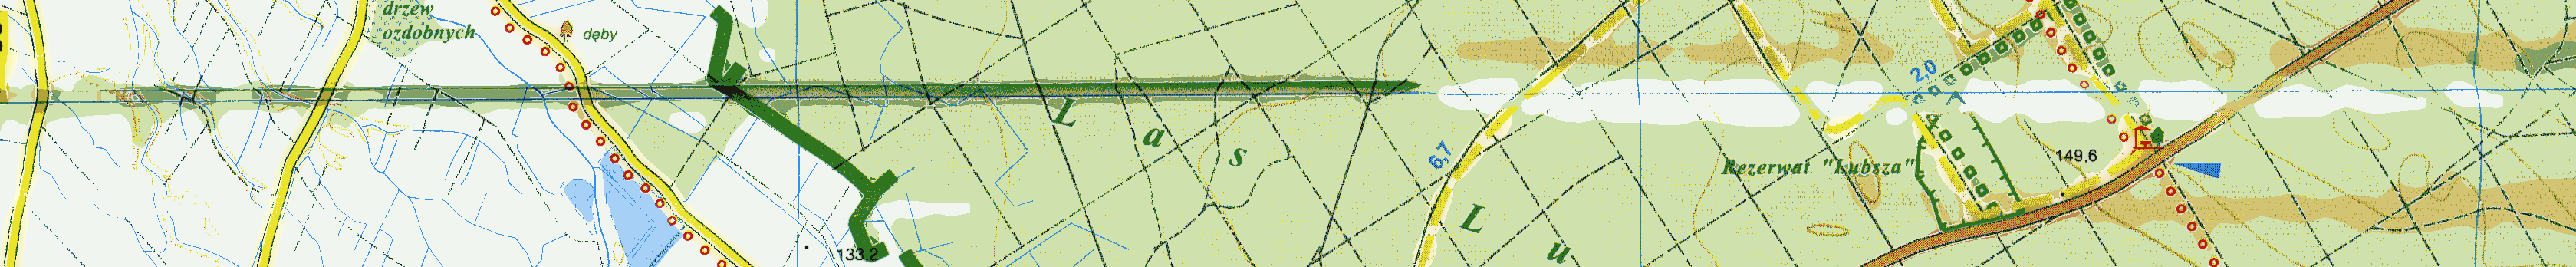
\includegraphics[scale=0.13]{images/lubszaCreased.png}
\caption{Input map crease visible in a segmented Lubsza map.}
\label{lubszaCreased}
\end{center}
\end{figure}

Performance of the algorithm is presented in a table \ref{lubszaPerformance}.

\begin{table}[!ht]
\begin{center}
\caption{Time of algorithm execution - Lubsza.}
\label{lubszaPerformance}
\begin{tabular}{|c|c|c|}
  \hline
  Detail Detection & Background Detection & Total Time \\
  \hline
  13 min 44s & 1h 12min 11s & 1h 12min 11s \\
  \hline
\end{tabular}
\end{center}
\end{table}

\subsection{Bydgoszcz}

Bydgoszcz is a city map. It has a lot of details (streets with names, small elements from a legend,
names of companies, ...). Additionaly it has many areas marked with different colors and a river
marked as a thick blue line. Maps has some distortions. It has visible creases and it is dirty.

\subsubsection{Used parameters}

All parameters used in this map have small values. It is caused by small resolution of the image. 
In background detection filtration, Gaussian blur radius is set to 5, bilateral filter diameter is
3, sigma space and sigma color is 50. Dilation and erosion is done once with size set to 1. Width
of a window is also small - it is set to 5. Background has maximum 15 colors. \\

Line detection is sensitive. Threshold is set to 100, which for small map is a big value. Similarly
to background detection part, all filters are applied with small parameter values. Unsharp mask
standard deviation is set to 1, denoising factor is 15. Bilateral filter is applied once with
diameter set to 5, sigma space and sigma color set to 50. Gaussian filter is also applied once with
radius set to 3. Map has many details. Maximum number of colors is set to 25, initial threshold is
10 and minimal color area is 500.

\subsubsection{Achieved results}

Achieved result with a map of Bydgoszcz is presented in a Fig.~\ref{bydgoszczResult}.

\begin{figure}[!ht]
\begin{center}
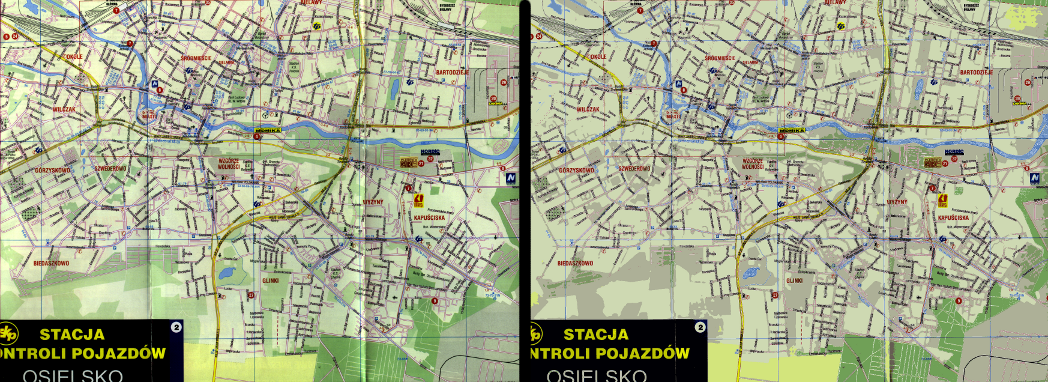
\includegraphics[scale=0.4]{images/bydgoszczFinalResult.png}
\caption{Final result of the algorithm applied to Bydgoszcz map. Input image is on the left, the
result is on the right side of an image.}
\label{bydgoszczResult}
\end{center}
\end{figure}

In case of the map of Bydgoszcz, the result of the algorithm is worse than achieved in other
images. Shape of the background areas is correct in most of cases, but due to small resolution of
the map and a lot of distortions, many areas are assigned to wrong groups. It is shown in a
Fig.~\ref{bydgoszczBadAreas}.

\begin{figure}[!ht]
\begin{center}
\includegraphics[scale=0.4]{images/bydgoszczBadAreas.png}
\caption{Areas assigned to wrong groups in a Bydgoszcz map.}
\label{bydgoszczBadAreas}
\end{center}
\end{figure}

Text and details remained readable, but in some places they are not as sharp as they were in the
input image. This situation is presented in a Fig.~\ref{bydgoszczBadSharpness}.

\begin{figure}[!ht]
\begin{center}
\includegraphics[scale=0.7]{images/bydgoszczBadSharpness.png}
\caption{Lost text sharpness in a Bydgoszcz map.}
\label{bydgoszczBadSharpness}
\end{center}
\end{figure}

Quality of the output image is the worst in case of a map of Bydgoszcz, but this situation is
probably caused by the quality of an input image.

Performance of the algorithm is presented in a table \ref{bydgoszczPerformance}.

\begin{table}[!ht]
\begin{center}
\caption{Time of algorithm execution - Bydgoszcz.}
\label{bydgoszczPerformance}
\begin{tabular}{|c|c|c|}
  \hline
  Detail Detection & Background Detection & Total Time \\
  \hline
  2 min 31s & 2min 24s & 2min 31s \\
  \hline
\end{tabular}
\end{center}
\end{table}

\subsection{Namysłów and Masyw Ślęży}

Namysłów and Masyw Ślęży are examples of topographic maps. They have a lot of very thin topographic
lines, small details and text. There are also marked cities and towns. Background of these images is
white. Only green areas, cities and lakes are marked in a different, bright colors.

\subsubsection{Used parameters}

Removal of details in a background detection algorithm is not a hard task in case of topographic
lines - details are very small. In this algorithm there is used strong filtration. Radius of a
Gaussian filter is set to 13. In Bilateral filter diameter is set to 10, sigma color and sigma
space to 150. Dilation and erosion is applied 5 times with size set to 1. Window width for holes
removal is set to 20. Maximum number of background colors for these maps is set to 10. \\

Line detection algorithm is very sensitive. It has to find all thin lines and small details or
letters. Threshold is big - it is set to 150. To improve the image quality, standard deviation for
unsharp mask is set to 3 and denoising factor to 35. Gaussian blur is applied once with a radius
set to 3. Bilateral filter is applied twice with a diameter set to 10, sigma color to 70 and sigma
space to 10. Maximum number of colors is set to 11, initial threshold is 10 and minimal color area
is 500.

\subsubsection{Achieved results}

The map of Namysłów with the algorithm applied is shown in a Fig.~\ref{namyslowResult}.

\begin{figure}[!ht]
\begin{center}
\includegraphics[scale=0.6]{images/namyslowResult.jpg}
\caption{Final result of the algorithm applied to Namysłów map. Input image is on the left, the
result is on the right side of an image.}
\label{namyslowResult}
\end{center}
\end{figure}

Namysłów map is segmented very well. Areas have the same borders, almost all pixels are assigned
to proper group. All small details and thin topographic lines are visible and sharp. Text is
readable. Resulting map has only small, hardly visible errors.

Performance of the algorithm is presented in a table \ref{namyslowPerformance}.

\begin{table}[!ht]
\begin{center}
\caption{Time of algorithm execution - Namysłów.}
\label{namyslowPerformance}
\begin{tabular}{|c|c|c|}
  \hline
  Detail Detection & Background Detection & Total Time \\
  \hline
  15 min 42s & 50min 17s & 50min 18s \\
  \hline
\end{tabular}
\end{center}
\end{table}

Results achieved with the map of Masyw Ślęży is presented in a Fig.~\ref{masywSlezyResult}.

\begin{figure}[!ht]
\begin{center}
\includegraphics[scale=0.8]{images/masywSlezyResult.png}
\caption{Final result of the algorithm applied to Masyw Ślęży map. Input image is on the left, the
result is on the right side of an image.}
\label{masywSlezyResult}
\end{center}
\end{figure}

Results of the test with the map of Masyw Ślęży is also very good. Borders of areas are properly
placed, text, details and thin topographic lines are visible and readable. Unfortunately in some
places color of the background is assigned wrongly. It can be seen in a Fig.~\ref{masywSlezyBadAreas}.

\begin{figure}[!ht]
\begin{center}
\includegraphics[scale=0.3]{images/masywSlezyBadAreas.png}
\caption{Wrongly assigned areas in a map of Masyw Ślęży.}
\label{masywSlezyBadAreas}
\end{center}
\end{figure}

Performance of the algorithm is presented in a table \ref{masywSlezyPerformance}.

\begin{table}[!ht]
\begin{center}
\caption{Time of algorithm execution - Masyw Ślęży.}
\label{masywSlezyPerformance}
\begin{tabular}{|c|c|c|}
  \hline
  Detail Detection & Background Detection & Total Time \\
  \hline
  16 min 11s & 53min 22s & 53min 23s \\
  \hline
\end{tabular}
\end{center}
\end{table}

\subsection{Dolny Śląsk}

Dolny Śląsk is old (from 1909) German map of Lower Silesia. There are marked main cities and towns
 (their names, borders) and rivers. This map has a lot of small elements (especially text) and
very thin lines. Moreover, map is damaged - it has some creases visible. Map has no background - 
there are only contours on a white background visible. 

\subsubsection{Used parameters}

The map of Dolny Śląsk does not have any background. The background detection part is disabled in
this case. Line detection must be very sensitive, because map contains a lot of very small details.
Thresholding for this map is set to 245. To improve image quality, there is used an unsharp mask
with standard deviation set to 1 and denosing algorithm with a factor value set to 20. Gaussian blur
is applied once with radius set to 1. Bilateral filter is applied twice with diameter set to 10,
sigma color to 70 and sigma space to 10. Maximum number of colors is set to 7, initial threshold
to 10 and minimum color area to 500.

\subsubsection{Achieved results}

Result of the algorithm application in a map of Dolny Śląsk is presented in a 
Fig.~\ref{dolnySlaskResult}.

\begin{figure}[!ht]
\begin{center}
\includegraphics[scale=0.2]{images/dolnySlaskResult.png}
\caption{Final result of the algorithm applied to Dolny Śląsk map. Input image is on the left, the
result is on the right side of an image.}
\label{dolnySlaskResult}
\end{center}
\end{figure}

This map is segmented very well. The text and small elements are visible and readable. Almost all,
even very thin lines are visible and have proper color set. Only one visible error is in places,
where map is creased. The algorithm is not able to eliminate these distorions and recognizes it
as a river. This situation is presented in a Fig.~\ref{dolnySlaskZagiecie}.

\begin{figure}[!ht]
\begin{center}
\includegraphics[scale=0.2]{images/dolnySlaskZagiecie.png}
\caption{Crease visible in a result map of Dolny Śląsk.}
\label{dolnySlaskZagiecie}
\end{center}
\end{figure}

\newpage

Performance of the algorithm is presented in a table \ref{dolnySlaskPerformance}.

\begin{table}[!ht]
\begin{center}
\caption{Time of algorithm execution - Dolny Śląsk.}
\label{dolnySlaskPerformance}
\begin{tabular}{|c|c|c|}
  \hline
  Detail Detection & Background Detection & Total Time \\
  \hline
  1h 29 min 10s & 1h 36min 51s & 1h 36min 52s \\
  \hline
\end{tabular}
\end{center}
\end{table}

\chapter{Conclusions}

In this Master Thesis, the filtration and segmentation algorithm for digital color scanned maps was
created. There was checked impact of many known filters and segmentation algorithms to this type of
images. In the basis of gained knowledge there were chosen the best found methods for digital maps
processing. To some of them there were applied needed modifications. Additionaly there was designed
a color-based segmentation algorithm for grouping map background and details by their type. As a
part of the work there was also an application developed, which was used in the method evaluation
process. Created algorithm was fully tested. In this process there were used nine different
 (topographic, geographical, city, old) maps. \\

Tests showed, that the algorithm gives good results, but not for every image. In case of 
geographical maps, like Ślęża, Sobótka or Pokój, background color was unified. Borders of all areas
remained unchanged and main details were kept. Additionaly many distortions were eliminated. Slighty
worse results were achieved with Lubsza and Brzeg. This was a consequence of some major distortions
existing these maps (like creases or darker elements) - the algorithm was not able to deal with these
types of difficulties. 

The algorithm gives quite good results also for topographic maps. Both
Namysłów and Masyw\_Ślęży output image quality was good. Small distortions were eliminated,
background color was unified and borders of areas were at the same place as in the input. The most
important in this type of maps - thin topographic lines and small elements and text were not damaged
after segmentation process.

In case of large old maps with a big number of small-sized elements and thin lines, like Dolny 
Śląsk, it is very difficult to set proper algorithm parameters. With that kind of map it is
difficult to combine the image quality (no distortions) and keeping all map details (especially a very
thin lines). In case of map of Dolny Śląsk, the algorithm recognized almost all elements properly.

The worst results were achieved with a map of Bydgoszcz. Many areas are damaged - they have wrong
shape and color and text is less readable than in the original. It can be caused by a very small
image resolution and presence of many distortions.

The main weakness of the algorithm is its performance. Time of preprocessing of bigger maps is very
long - it takes more than one hour. It is caused by the number of operations which should be
executed for each pixel. The slowest parts of the whole procedure are Bilateral Filter and
segmentation algorithm. Another disadvantage is a number of parameters, which have to be adjusted
for every map.\\

The algorithm in this form gives good results for many types of maps. However it is suitable for
further development. The improvements can be done in a field of background detection (especially with
a city maps, like Bydgoszcz) and better removal of distortions. Moreover, another class distance
measurement algorithms can be tested (for example Mahalanobis distance instead of Euclidean
distance) Additionaly, pre-analysis of the input map can be added to eliminate, or at least reduce
the number of parameters. The work should be also focused on execution time of the algorithm. The
short execution time was not main aim of this work (the algorithm will not work as the real-time
apllication), however improvement on this field would ease testing process. Another improvement,
which would improve the convenience of the application usage would be a GUI development.
In the field of testing, it is a very good idea to test results of this algorithm by specialised
software. Unfortunately it was not possible to carry out this type of tests in this work. \\

The presented algorithm is a variant of color scanned maps segmentation. With properly set
parameters it is a good way to process this type of digital images.

\newpage

\renewcommand\bibname{References}

\begin{thebibliography}{   }

	\bibitem{digitalImageProcessing}
          {Rafael C. Gonzalez, Richard E. Woods, Digital Image Processing, Prentice Hall, 3rd Edition, 2007}
  \bibitem{learningOpenCv}
          {Gary Bradski, Adrian Kaehler, Learning OpenCV. Computer Vision with the OpenCV Library,
          O`Reilly Media Inc., 2008}
  \bibitem{bilateralFilterWiki}
          {http://en.wikipedia.org/wiki/Bilateral\_filter, Version from 29.05.2014}
  \bibitem{unsharpMaskWiki}
          {http://en.wikipedia.org/wiki/Unsharp\_masking, Version from 1.06.2014}
  \bibitem{nonLocalMeansDenoising}
          {http://www.ipol.im/pub/art/2011/bcm\_nlm/, Version from 1.06.2014}
  \bibitem{semanticAnalysisAndRecognition}
          {Serguei Levachkine, Aurelio Velázquez, Victor Alexandrov, Mikhail Kharinov, 
          Semantic Analysis and Recognition of Raster-Scanned Color Cartographic Images,
          4th International Workshop, GREC 2001 Kingston, Ontario, Canada, September 7–8, 
          2001 Selected Papers, 2002}
  \bibitem{comparativeAnalysisOfScannedMaps}
          {C. Armenakis, F. Leduca, I. Cyra, F. Savopola, F. Cavayasb,
          A comparative analysis of scanned maps and imagery for mapping applications,
          ISPRS Journal of Photogrammetry and Remote Sensing Volume 57, Issues 5–6, April 2003,
          Pages 304–314}
  \bibitem{colorsOfThePast}
          {Stefan Leyk, Ruedi Boesch, Colors of the past: color image segmentation in historical 
          topographic maps based on homogeneity, GeoInformatica, January 2010, Volume 14, Issue 1, pp 1-21 }
  \bibitem{automaticVectorization}
          {Huali Zheng, Xianzhong Zhou, Hongbo Wang, Automatic Vectorization of Contour Lines Based
          on Deformable Model with Adaptive Flow Orientation, Proceedings of the 2003 IEEE
          International Conference on Robotics,Intelligent Systems and Signal Processing
          Changsha, China - October 2003}
  \bibitem{topographicMapsAutomaticVectorization}
          {Marc Pierrot Deseilligny, Robert Mariani, Jacque Labiche, Remy Mullot,
          Topographic Maps Automatic Interpretation: Some Proposed Strategies, Second International
          Workshop, GREC' 97 Nancy, France, August 22–23, 1997}
  \bibitem{colorMapSegmentation}
          {Alireza Khotanzad, Edd Zink, Color paper map segmentation using eigenvector line-fitting,
          Image Analysis and Interpretation, 1996., Proceedings of the IEEE Southwest Symposium on
          8-9 April 1996}
  \bibitem{cmakeMainPage}
          {http://www.cmake.org/, Version from 17.06.2014}
  \bibitem{opencvMainPage}
          {http://opencv.org/, Version from 17.06.2014}
  \bibitem{boostWiki}
          {http://en.wikipedia.org/wiki/Boost\_\%28C\%2B\%2B\_libraries\%29, Version from 17.06.2014}
  \bibitem{boostMainPage}
          {http://www.boost.org/, Version from 17.06.2014}
  \bibitem{stlWiki}
          {http://en.wikipedia.org/wiki/Standard\_Template\_Library, Version from 18.06.2014}
  \bibitem{rapidXmlMainPage}
          {http://rapidxml.sourceforge.net/, Version from 18.06.2014}
  \bibitem{imageScanner}
          {http://en.wikipedia.org/wiki/Image\_scanner, Version from 25.06.2014}
  \bibitem{gestaltTheory}
          {From Gestalt Theory to Image Analysis, Agnes Desolneux, Lionel Moisan, Jean-Michel Morel,
          10 July 2006}
  \bibitem{cmykWiki}
          {http://en.wikipedia.org/wiki/CMYK\_color\_model, Version from 28.06.2014}
  \bibitem{halftoneWiki}
          {http://en.wikipedia.org/wiki/Halftone, Version from 28.06.2014}
}

\end{thebibliography}

\end{document}
